\documentclass[10pt]{article}

\usepackage[margin=0.78in]{geometry}
\usepackage{amsmath,amssymb,mathtools}
\usepackage{booktabs,longtable,tabularx,array,multirow}
\usepackage{graphicx}
\usepackage{xcolor}
\usepackage{microtype}
\usepackage{enumitem}
\usepackage{caption}
\usepackage{fancyhdr}
\usepackage[hidelinks]{hyperref}
\usepackage{xurl}
\usepackage{xspace}

\definecolor{sidblue}{HTML}{174A7E}
\definecolor{sidlight}{HTML}{EAF1F8}
\definecolor{sidred}{HTML}{8E2C2C}
\definecolor{sidgreen}{HTML}{2C6E49}
\definecolor{sidgray}{HTML}{5D6570}

\hypersetup{
  colorlinks=true,
  linkcolor=sidblue,
  citecolor=sidblue,
  urlcolor=sidblue,
  pdftitle={Stable Finite SID: Theory, Adversarial Synthetic Evidence, and Decision Rules},
  pdfauthor={diffusionCircuit project synthesis}
}

\setlist[itemize]{leftmargin=1.35em,itemsep=2pt,topsep=4pt}
\setlist[enumerate]{leftmargin=1.55em,itemsep=3pt,topsep=4pt}
\setlength{\parindent}{0pt}
\setlength{\parskip}{5pt}
\renewcommand{\arraystretch}{1.16}

\pagestyle{fancy}
\fancyhf{}
\lhead{Unified SID synthesis}
\rhead{13 July 2026}
\cfoot{\thepage}
\setlength{\headheight}{13pt}

\newcommand{\Ph}{P_h}
\newcommand{\E}{\mathbb{E}}
\newcommand{\R}{\mathbb{R}}
\newcommand{\given}{\,\middle|\,}
\newcommand{\nise}{\operatorname{nISE}}
\newcommand{\nrmse}{\operatorname{NRMSE}}
\newcommand{\SIDQ}{\textnormal{\textsc{SID-Q}}\xspace}
\newcommand{\FiniteSID}{\textnormal{\textsc{Finite-SID}}\xspace}
\newcommand{\DiffSID}{\textnormal{\textsc{Diffusion-SID}}\xspace}
\newcommand{\SBTGK}{\textnormal{\textsc{SBTG-K}}\xspace}
\newcommand{\CPSID}{\textnormal{\textsc{CP-SID}}\xspace}
\newcommand{\yes}{\textcolor{sidgreen}{yes}}
\newcommand{\no}{\textcolor{sidred}{no}}

\newenvironment{takeaway}
  {\begin{quote}\color{sidblue}\textbf{Bottom line.}\ }
  {\end{quote}}

\title{\vspace{-1.2cm}\textbf{Stable Finite SID}\\[3pt]
\large Theory, adversarial synthetic evidence, failure diagnosis, and decision rules}
\author{Internal methods synthesis for the diffusionCircuit project}
\date{13 July 2026}

\begin{document}

\maketitle

\begin{abstract}
The project has accumulated several methods that initially look separate: quadratic score-based interaction discovery, the original score-based temporal graph operator, point-history tangents, finite history contrasts, conditional diffusion, and channel-specific changepoint scans. They are better understood as components of one program. The population object is the observed conditional predictive law \(h\mapsto P(Y\mid H=h)\). A predictive backend represents that law by a normalized density, an outcome score, a joint-state score, or samples. An adapter converts the representation into a supported history contrast or derivative. A typed readout declares whether the target is mean, dispersion, covariance, interaction, skewness, or tail behavior. A calibrated inference layer can then detect static structure or temporal changes.

This synthesis audits the recent synthetic experiments under that decomposition and then replaces the weakest synthetic lane with exact, adversarial conditional laws. The empirical conclusion is candid. Normalized likelihood and classical sparse dynamics remain the leaders when their models are tractable and approximately correct. Outcome-space denoising score matching, history-score SID, and flow velocity are different mathematical objects; a good denoising loss does not by itself estimate SID. The earlier neuromodulator stress suite also contains decisive implementation and comparison defects, including a non-operative E3 shift, deterministic ``stochastic'' release, marginal rather than joint density scoring, and unequal method cell sets. Its rankings are therefore diagnostic rather than adjudicative.

The recommended research direction is \emph{finite, typed, support-aware SID}: form an exact finite signed contrast at a scientifically declared perturbation scale; estimate bounded or projected witnesses through multiple routes; and report channel-specific functionals with route-agreement and mechanism-confusion controls.  On the new exact whole-future-path law, a raw path classifier recovers a pure fourth-order effect to 3.05\% median error while linear and quadratic routes recover none.  Full-law diffusion, flow, and autoregressive samplers recover only 0--6\% of that effect.  Classifier guidance of a frozen midpoint generator is a partial repair---EDM rises from 1\% to 40\% effect slope---but does not replace the higher-order geometry the generator discarded.  Explicit endpoint experts under the same total data budget also help EDM, but only to 34\% slope.  The evidence therefore favors a normalized global mixture gate or finite ratio/classifier head \emph{and} topology-aligned expert training, with diffusion or flow used only for residual within-mode geometry.  Exact-rejection bounded energy, frozen-anchor stochastic interpolation, and an 80-cell endpoint-expert factorial make that conclusion testable rather than architectural speculation.
\end{abstract}

\tableofcontents
\newpage

\section{July 13 adversarial revision: what changed}

\begin{takeaway}
The main problem was not one thing.  The quadratic SID failures are partly structural; the first neuromodulator stress suite also had invalid or missing experimental axes; and several comparisons conflated predictive-law backends with SID estimators.  The repaired program keeps finite typed SID as the estimand, uses normalized densities, bounded energies, diffusion, and flow only as alternative backends, and tests all routes on exact laws designed to conceal changes from mean and covariance baselines.
\end{takeaway}

Four corrections govern the rest of this report.

\begin{enumerate}
  \item \textbf{Derivative types are not interchangeable.}  Diffusion DSM targets
  $\nabla_y\log p_\sigma(y\mid h)$; infinitesimal SID targets
  $D_v\log p(y\mid h)$; flow matching targets a transport velocity in artificial
  time.  A diffusion or flow can support finite SID through samples, but its native
  vector field is not itself the SID witness.
  \item \textbf{The original quadratic DSM parameterization is inadmissible.}
  If an affine noisy score has precision $B_\sigma$, a positive clean Gaussian
  covariance requires $0\prec B_\sigma\prec\sigma^{-2}I$.  Free affine natural
  parameters do not enforce this spectral interval and cannot remain in a bounded
  interval globally over an unbounded history space.
  \item \textbf{The earlier E3/E4 neuromodulator evidence is downgraded.}  The E3
  reservoir branch ignored the declared state-mixture shift, so its two OOD levels
  were bit-identical.  E4's release was deterministic conditional on state.  Neural
  and classical rankings also averaged unequal cell sets, and response RMSE was
  scaled by overall signal variation rather than the intervention-effect scale.
  \item \textbf{A real home field must hide changes from low-order baselines.}  The
  new exact path law changes only higher-order multimodal topology along its declared
  contrast direction; its conditional mean and covariance are invariant.  Gaussian
  methods therefore cannot win merely because the target is mean-like, while exact
  density, score, ratio, and sampling oracles remain available.
\end{enumerate}

\subsection{The revised method stack}

The operative scientific object is
\[
  \boxed{\text{predictive-law backend}
  \longrightarrow\text{finite signed contrast}
  \longrightarrow\text{typed readout}
  \longrightarrow\text{dynamic/interventional aggregation}.}
\]
The layers have different validation obligations.  A held-out NLL or energy score
validates a backend; witness calibration validates a contrast adapter; channel RMSE
validates a typed readout; and rollout or changepoint error validates aggregation.
No native training loss substitutes for the downstream gate.

\subsection{Bounded finite SID theorem}

For histories $h_1,\ldots,h_R$, signed coefficients $c_r$ with $\sum_r c_r=0$,
and $C=\sum_r|c_r|$, define
\[
  \nu_c=\sum_r c_rP_{h_r},\qquad
  M_c=\sum_r\frac{|c_r|}{C}P_{h_r},\qquad
  W_c=\frac{d\nu_c}{dM_c}.
\]
Then $\nu_c\ll M_c$ even if the contrasted laws are mutually singular,
$|W_c|\leq C$, $E_{M_c}W_c=0$, and
\[
  \sum_r c_rE_{P_{h_r}}\phi(Y)=E_{M_c}\{\phi(Y)W_c(Y)\}
\]
for every integrable $\phi$.  If a label $R$ is drawn with
$\Pr(R=r)=|c_r|/C$ followed by $Y\sim P_{h_r}$, then the calibrated posterior
$\pi_r(y)=\Pr(R=r\mid Y=y)$ gives
\[
  W_c(y)=C\sum_r\operatorname{sign}(c_r)\pi_r(y).
\]
For a central first difference this becomes
\[
  W_\delta(y)=\delta^{-1}\{2\eta(y)-1\}
  =\delta^{-1}\tanh\!\left\{\tfrac12\log(p_+(y)/p_-(y))\right\}.
\]
Thus the recommended finite witness is a bounded transform of a potentially
unbounded density ratio.  With excess classifier log loss $\mathcal R_{\log}$,
Pinsker's inequality yields
\[
 E_{M_c}(\widehat W_c-W_c)^2\leq2C^2\mathcal R_{\log},
\]
which makes calibration a quantitative SID diagnostic rather than an optional
classifier statistic.  The ratio--class-probability link is also the basis of
proper-composite density-ratio estimation \cite{menon2016}.

\subsection{Direct readouts and common-random-number coupling}

For one predeclared $\phi$, the direct group-mean contrast is generally more
efficient than learning an omnibus witness.  The omnibus witness earns its cost
when many readouts are queried, response-space localization is itself scientific,
or one shared backend interpolates many histories.  Generators also permit a useful
coupling: with $Y_\pm=G(h_\pm,Z)$ and the same latent $Z$,
\[
 \widehat\Delta_{\mathrm{pair}}
 =\frac1n\sum_i
 \frac{\phi\{G(h_+,Z_i)\}-\phi\{G(h_-,Z_i)\}}{2\delta}.
\]
If the paired numerator is $O_{L^2}(\delta)$, the variance is $O(n^{-1})$ rather
than the generic independent-sample $O\{(n\delta^2)^{-1}\}$.  This coupling,
not the native diffusion loss, is one plausible advantage of flow and diffusion
backends.

\subsection{When classifier guidance can repair a generator}

For a balanced two-history contrast, let
$M=(P_++P_-)/2$ and $\eta(y)=\Pr(Z=+\mid Y=y)$.  The exact identities
\[
  \frac{dP_+}{dM}=2\eta,
  \qquad
  \frac{dP_-}{dM}=2(1-\eta)
\]
give a constructive global-mass head.  If a generator draws exactly from $M$,
self-normalized reweighting by $\widehat\eta$ and $1-\widehat\eta$ recovers the
two endpoint laws when the classifier is calibrated.  This is the finite-SID
analogue of guidance, but it has a sharper target than multiplying a conditional
score difference.

The construction also separates two errors.  Write $Q$ for the learned midpoint
law, with densities $q,m$, and let
$\widehat P_+\propto\widehat\eta q$.  If
$A=\int\widehat\eta q\geq\kappa>0$, then
\[
 \operatorname{TV}(\widehat P_+,P_+)
 \leq \kappa^{-1}\|\widehat\eta q-\eta m\|_1
 \leq \kappa^{-1}\left\{
 E_Q|\widehat\eta-\eta|+\int\eta|q-m|
 \right\}.
\]
The first term is contrast-head error; the second is midpoint-generator geometry
error.  Hence even a Bayes classifier cannot recover a fourth-order component
that is absent from $Q$.  Conversely, fitting a perfect generator without a
contrast-aligned head leaves the global mass derivative unidentified in the
separated-support limit.  This decomposition motivates a statistical
mixture-of-transports rather than post-hoc guidance alone.

\subsection{A stable score-to-SID bridge}

For an energy law $p_\theta(y\mid h)\propto\exp\{-E_\theta(y,h)\}$,
\[
 D_v\log p_\theta(y\mid h)
 =-D_vE_\theta(y,h)+E_{p_\theta}\{D_vE_\theta(Y,h)\}.
\]
The partition function cancels after conditional centering.  The implemented
tail-safe version starts from a normalized Gaussian reference $q_\psi$ and uses
\[
 p_{\theta,\psi}(y\mid h)
 \propto q_\psi(y\mid h)
 \exp\{B\tanh f_\theta(y,h)\}.
\]
It inherits the reference tails, has importance weights in $[e^{-B},e^B]$, is
curl-free in response space, and exposes a centered history derivative.  This is
a direct theoretical bridge from non-normalized score modeling to SID.  An
unconstrained denoiser does not have the same property.

The distinction between the law and its numerical sampler is essential.  The
initial implementation draws a finite pool from $q_\psi$ and resamples using
softmax weights.  That is sampling--importance resampling: it is finite-pool
biased and repeated outputs share the proposal pool.  Its draws therefore do not
satisfy the independence assumption used by the fair finite-ensemble energy
score, and its current proper-score rows are excluded from primary rankings.  A
bounded tilt admits an exact replacement.  If $Y^\star\sim q_\psi(\cdot\mid h)$
and $U\sim\operatorname{Unif}(0,1)$, accept when
\[
  \log U\leq B\tanh f_\theta(Y^\star,h)-B.
\]
Accepted proposals are i.i.d. from $p_{\theta,\psi}$, with acceptance
$e^{-B}Z(h)\geq e^{-2B}$.  Thus $B$ controls a genuine approximation--computation
tradeoff: larger $B$ reduces ratio clipping but can make exact sampling and
importance centering exponentially inefficient.  Confirmation requires exact
rejection draws, conditional acceptance and proposal-cap diagnostics, and
agreement between exact centering and a separately reported self-normalized
importance estimate.

The exact sampler is now implemented and validated against analytic tilted
Gaussians.  Reevaluation of all 64 frozen bounded-energy checkpoints completes
without failure: empirical median acceptance is 0.136--0.431 across laws and
proposal materialization never exceeds the 4,096 cap.  Its fair energy is
competitive but not generally best, and its G8 quartic slope is essentially zero.
Thus the bridge is mathematically and computationally viable, but the current
ratio-versus-Gaussian training objective still does not allocate signal to the
hard conditional mass channel.

An objective-controlled score comparison also freezes one Gaussian reference and
fits the same bounded tilt by conditional Hyv\"arinen loss,
\[
 E\!\left[\tfrac12\|s_q+\nabla_yu\|^2+
 \nabla_y\!\cdot s_q+\Delta_yu\right],
 \qquad u=B\tanh f_\theta.
\]
This isolates clean response-score fitting from classifier ratio fitting.  It is
expected to favor smooth within-mode shape changes, whereas a calibrated ratio
classifier should retain an advantage when only separated component masses
change.  Neither objective is licensed as a history-SID estimator until the
centered history derivative is validated downstream.

\subsection{Why SBTG can be intrinsically ill-conditioned}

SBTG's ideal mixed object $K_v=D_v\nabla_y\log p_h=\nabla_y\ell_v$ recovers
only the response gradient of the history witness.  If $P_h$ satisfies a
Poincar\'e inequality with constant $C_P$ and a centered reconstruction obeys
$\|\nabla\widehat\ell-K_v\|_{L^2(P_h)}\leq\epsilon$, then
\[
 \|\widehat\ell-\ell_v\|_{L^2(P_h)}\leq\sqrt{C_P}\,\epsilon.
\]
Separated mixtures can have enormous $C_P$; disconnected support leaves one
unknown constant per component.  Consequently, clean outcome scores may barely
change when only mixture weights change.  This is a theoretical home-field for
finite classifiers and ratios, and a structural limitation of score-gradient
reconstruction rather than merely a training failure.

The limiting case makes the obstruction exact.  Let

\[
 p_a(y)=\sum_{k=1}^K\pi_k(a)f_k(y),
 \qquad \operatorname{supp}(f_j)\cap\operatorname{supp}(f_k)=\varnothing
 \quad(j\ne k),
\]

where the component laws are fixed and only their history-dependent masses
$\pi_k(a)$ vary.  For $y\in\operatorname{supp}(f_k)$,

\[
 \nabla_y\log p_a(y)=\nabla_y\log f_k(y),
 \qquad
 \partial_a\log p_a(y)=\partial_a\log\pi_k(a).
\]

Thus every history has exactly the same clean outcome-score field even though
its SID witness is nonzero and can be large.  Clean Hyv\"arinen or denoising
score matching cannot infer the missing component constants from within-component
gradients.  With Gaussian corruption, the supports overlap and the obstruction
becomes an ill-conditioning result rather than non-identification: the conditional
score difference is concentrated in the low-probability frame-ambiguity region.
Increasing $\sigma$ first exposes that region and then erases the original law
contrast.  A generic average over noise levels can therefore achieve a low DSM
loss while allocating almost no effective signal to history-controlled mode
mass.

This proposition also explains why the appropriate repair is not simply a larger
denoiser.  A full backend for this regime needs a global-mass channel: a normalized
mixture gate, a calibrated finite classifier, a density-ratio or bounded-energy
head, or an equivalent contrast-aligned auxiliary loss.  Diffusion or flow can
still model the conditional geometry within components, but the gate or ratio
head must carry the component constants that local outcome scores discard.

\subsection{Stabilization implemented in the new benchmark}

The new backend panel includes: (i) clean-covariance Gaussian parameterization
trained by NLL or multiscale DSM; (ii) an exact conditional affine flow;
(iii) EDM input/output/skip preconditioning, log-normal noise sampling, a
$\rho=7$ schedule, and Heun integration; (iv) EDM anchored around a learned
conditional Gaussian mean and scale; (v) ordinary and Gaussian-source conditional
flow matching; and (vi) the bounded energy tilt above.  These changes follow the
separation and preconditioning principles of EDM \cite{karras2022}, the
simulation-free vector regression of flow matching \cite{lipman2023}, and the
Gaussian-reference geometry needed for function-space diffusion \cite{lim2023}.
Whole-path operator methods are reserved for an actual
trajectory-valued response, not used merely because the conditioner is a time
series.

The literature suggests several additional stabilizers, but they address
different failure modes.  Stable Target Field replaces a single noisy DSM target
by an importance-weighted reference-batch average and specifically reduces target
variance in the ambiguous intermediate-noise regime \cite{xu2023stf}.  On G8 it
should be tested with reference batches stratified by declared control; it can
reduce variance near the visibility peak, but it cannot recover component masses
from clean within-component gradients.  Data-dependent or Gaussian-process source
laws shorten the transport and preserve temporal covariance, as in TSFlow
\cite{kollovieh2024}; a single Gaussian source still matches only first- and
second-order structure and therefore needs a ratio or mixture-gate head for the
pure fourth-order lane.  Denoising diffusion operators supply the correct
Gaussian-reference/Cameron--Martin geometry for whole functions \cite{lim2023},
but do not change the statistical estimand.  Stochastic interpolants supply a
non-singular conditional transport and post-training diffusion choice
\cite{chen2024}, but likewise require a contrast diagnostic to establish that
conditioning is actually used.

These observations define a minimal stabilization factorial rather than an
unstructured architecture search:

\begin{enumerate}
  \item EDM preconditioning and ordinary loss weighting;
  \item topology-window noise stratification, centered near the empirically
  visible intermediate scales;
  \item the same schedule with a control-stratified Stable Target Field;
  \item an auxiliary balanced finite-contrast classifier or bounded energy-ratio
  head, cross-fitted and calibrated;
  \item a statistical mixture-of-transports backend with a normalized
  history-dependent gate and diffusion/flow experts within modes.
\end{enumerate}

Items 2--3 test numerical/statistical stabilization of the local score.  Items
4--5 add the global mass information that the separated-support proposition says
is absent from that score.  Only the latter can be expected to solve a pure
mode-weight SID problem in the disjoint-support limit.  A classifier-free guidance
scale by itself is not a substitute: multiplying a nearly zero conditional score
difference does not create the missing per-component constants.

The controlled transport experiment uses a conditional point-source
stochastic interpolant, following the forecasting construction of Chen et
al.\ \cite{chen2024}.  With a frozen Gaussian conditional-mean anchor $a(h)$,
standardized response $y$, and $\xi\sim N(0,I)$, compare only
\[
 I_t=(1-t)a(h)+\beta_t y+(1-t)\sqrt t\,\xi,
 \qquad
 R_t=-a(h)+\dot\beta_t y-\sqrt t\,\xi,
\]
for $\beta_t=t$ versus $\beta_t=t^2$.  The latter has $\dot\beta_0=0$ and is
designed to remove a difficult initial transport impulse.  Its native sampler is
the Euler--Maruyama SDE
\[
 dX_t=b_\theta(X_t,t,h)\,dt+(1-t)dW_t,
 \qquad X_0=a(h).
\]
The apparently unusual $-\sqrt t\,\xi$ target is the forward-SDE drift, not the
raw time derivative of the interpolation noise.  With
$\gamma_t=(1-t)\sqrt t$ and diffusion $g_t=1-t$, the score correction gives
$\dot\gamma_t\xi-g_t^2\xi/(2\gamma_t)=-\sqrt t\,\xi$.  The implementation and
tests lock this identity, $\epsilon=1$, and the 128-step primary protocol.
This is a sampler-backend experiment, not a new SID definition.  The primary
comparison uses 128 steps with 64/256-step resolution checks.  All 32 frozen-anchor
fits completed.  Squared $\beta$ improves G8 fair energy from 0.717 to 0.710 but
reduces the already tiny quartic effect slope from 0.0075 to 0.0007; all three
sampler resolutions agree.  On the Gaussian G1 lane both schedules retain a real
mean effect (NRMSE 0.338/0.319).  Thus the G8 result is not an unstable sampler or
initial transport impulse.  Better transport conditioning improves a coarse law
metric while leaving the missing conditional mass statistic unresolved.

A final endpoint-expert factorial tests whether an explicit normalized gate alone
is sufficient.  It crosses four systems, two data seeds, two model seeds, and five
backend families.  Each method receives 8,000 total training examples, split
4,000/4,000 between the supported $-1/+1$ experts; the declared control is removed
from expert inputs and a deterministic gate selects the endpoint expert.  All 80
cells complete.  Relative to shared balanced-control fits, slopes increase to
0.336 for EDM, 0.251 for affine flow, 0.179 for MDN, and 0.035 for flow matching;
Gaussian remains zero.  This establishes that explicit gating helps, but the best
NRMSE is still 0.665.  The next architecture therefore needs both a normalized
gate and a contrast/topology-aligned expert loss; ordinary proper-law or transport
losses remain insufficient at this budget.

\subsection{Exact whole-path falsification law}

The new G8 response is a flattened multichannel future path.  Let
$U\in\mathbb R^{d\times r}$ be orthonormal traveling-wave motifs and let
\[
 \mathcal Z_A=\{\pm\sqrt r e_i\}_{i=1}^r,
 \qquad
 \mathcal Z_B=\{\pm\sqrt r R e_i\}_{i=1}^r
\]
for a non-axis-aligned orthogonal $R$.  Both frames have mean zero and covariance
$I_r$.  Given nonlinear observed history $h$, a stable path mean $m(h)$, correlated
noise $C_0$, and a declared shape control $a(h)$, G8 uses
\[
 Y\mid h,z\sim N\{m(h)+\alpha Uz,C_0\},\qquad
 \Pr(z\in\mathcal Z_B\mid h)=\operatorname{logit}^{-1}\{1.2a(h)\}.
\]
Changing the declared control changes mixture topology and higher moments while
mean and covariance remain exactly invariant.  The law is a finite Gaussian
mixture with exact clean/noisy log density, response score, history tangent, finite
ratio, and conditional sampler.  This is the decisive synthetic lane for whether
a flexible joint-law backend and finite SID adapter can expose scientifically typed
path changes that Gaussian baselines erase.

The readout must match the construction.  A dictionary ending at cubic order is
blind by design to much of this symmetric, moment-matched signal.  The corrected
panel includes an exact frame-occupancy readout and a noise-adjusted fourth-order
motif contrast.  With $u=U^\top\{Y-m(h)\}$, use a contrast of terms
\[
 H_4(x;s^2)=x^4-6s^2x^2+3s^4
\]
in the original and rotated motif frames.  Linear and quadratic path features are
predeclared negative controls, not weak positive targets.  An exact Gaussian
shadow $N\{m(h),C_0+\alpha^2UU^\top\}$ is run beside G8 with the same histories;
it matches G8's conditional first two moments but has identically zero shape
contrast.  In eight balanced-classifier negative-control cells its median AUC is
0.499 (range 0.496--0.505), and the largest spurious classifier-projected quartic
effect is 0.16\% of the corresponding positive G8 effect.  The successful G8
classifier is therefore not reading a mean/covariance mismatch or the control
label itself.

The first nonlinear-measurement draft is not admissible evidence: it corrupts only
future outputs while giving every model the latent history, and it restarts the
calcium, bleaching, and artifact processes at the prediction origin.  The repaired
experiment generates joint measured histories and futures, carries measurement
state across the boundary, appends missingness and time-since-observation, and
separates a declared-operator transfer task from an unannounced target-law shift.
Because $p(Y\mid H_{\mathrm{obs}})$ is not analytically available, this lane uses
proper scores on independent joint episodes and population randomized-operation
contrasts; pointwise oracle SID remains confined to the clean latent lane.

\subsection{What backend error can and cannot guarantee}

For a reverse diffusion with scalar diffusion coefficient $g_t$, common terminal
law, exact score $s_t$, and estimated score $\widehat s_t$, the usual Girsanov
conditions give a path-space KL proportional to
\[
 \frac12\int g_t^2E\|s_t-\widehat s_t\|^2dt.
\]
Data processing and Pinsker therefore bound terminal expectation error for
bounded $|\phi|\leq B$ by
\[
 \left|E_{P_0}\phi-E_{\widehat P_0}\phi\right|
 \leq B\left\{\int g_t^2E\|s_t-\widehat s_t\|^2dt\right\}^{1/2}.
\]
This supports integrated, noise-weighted score diagnostics for sampling.  It does
not imply accurate $D_h\log p$, and a small native DSM average can conceal the
intermediate-noise scales that carry mixture-weight information.

For flow matching, couple the true and learned ODEs with the same source draw.
If both velocities are $L$-Lipschitz, Gr\"onwall's inequality yields a
Wasserstein endpoint bound of the form
\[
 W_2(P_h,\widehat P_h)
 \leq\int_0^1 e^{L(1-t)}
 \{E\|v_t(X_t,h)-\widehat v_t(X_t,h)\|^2\}^{1/2}dt.
\]
Lipschitz readouts inherit this error.  Again, velocity MSE alone does not control
history derivatives of the flow.  The primary SID interface remains paired finite
samples unless normalized CNF likelihood is actually integrated.

\subsection{Function-space scope}

The finite signed-measure definition does not require Euclidean response space;
$M_c$ and $W_c=d\nu_c/dM_c$ exist on abstract path and function spaces.  A
function-space diffusion is more delicate: there is no infinite-dimensional
Lebesgue density, the score is defined relative to a Gaussian reference in
Cameron--Martin geometry, and the corruption covariance must be trace class.
Denoising diffusion operators therefore motivate GP/AR corruption and neural
operators only when $Y$ is an entire future trajectory or field.  They do not
make an ordinary one-step vector SID estimator more identified.  This distinction
is why the new benchmark first uses a finite exact path grid, then adds a
sample-only nonlinear measurement view and reserves resolution-transfer tests for
a later operator experiment.

\subsection{Frozen advancement rules}

A flexible generative backend advances only if it improves a held-out proper law
score over the strongest normalized baseline, beats both the autoregressive density
and conditional flow on a hard law, remains non-inferior on the Gaussian sanity law,
and has stable sampler resolution.  A score-derived SID adapter advances only if it
normalizes, centers, maintains usable importance-sampling ESS, satisfies the SID
moment identity, and improves on direct paired channels or calibrated classifier
ratios for at least two non-mean readouts.  Otherwise the generator may remain useful
while the score-based SID claim is rejected.

\section{Executive verdict}

\begin{takeaway}
There is no evidence that an outcome-score or diffusion objective is currently
the best general estimator of conditional dynamics.  The best-developed original
idea is finite, typed, support-aware SID.  It now succeeds not only for location
and low-rank occupancy changes but also for the audited whole-path fourth-order
G8 effect when trained as a calibrated finite classifier.  The same effect is
almost absent from full-law diffusion, flow, and autoregressive samplers despite
excellent marginal likelihood.  The immediate research program is therefore a
contrast-aligned ratio/energy or normalized mixture-gate head, with diffusion or
flow used for within-mode path geometry when that flexibility is actually needed.
\end{takeaway}

The main conclusions are:

\begin{enumerate}
  \item \textbf{The methods are not six independent theories.} They share one population object, \(P_h=P(Y\mid H=h)\), and differ mainly in representation, adapter, readout, and inference layer.
  \item \textbf{SID should be the umbrella, not the quadratic implementation.} The current closed-form quadratic model is denoted \SIDQ. It is one convenient score-matching backend with Gaussian reconstruction, not the definition of SID.
  \item \textbf{Finite contrasts are the most promising core.} They define an exact, supported comparison of predictive laws and can be estimated from densities, density ratios, classification, scores, or samples. This is the natural generalization of infinitesimal SID.
  \item \textbf{SBTG is a derivative/localization route, not a separate mechanism estimator.} Its ideal mixed operator is \(K_v=D_v\nabla_y\log p_h=\nabla_y D_v\log p_h\). Recovering the history witness from this gradient requires integration, centering, support, and boundary conditions. Current empirical SBTG statistics are reduced-form screens and are not mechanism-specific.
  \item \textbf{Diffusion and stochastic interpolation are backends.} They are useful if the law is complex, the normalizer is unavailable, or sampling is required. Denoising score matching targets a corrupted outcome score and stochastic interpolation a transport drift; neither by itself identifies the clean history derivative or a physical mechanism.  The new interpolant is stable on G1 yet has essentially zero G8 quartic slope at every tested sampler resolution.
  \item \textbf{Changepoints are an inference wrapper.} A changepoint scan can be applied to a validated mean, variance, tail, or general-law statistic. It does not rescue an invalid static channel.
  \item \textbf{Current wins are narrow but real.} Finite signed classifiers/ratios recover location changes, ratio critics recover low-rank mixture interactions, and a contrast-aligned classifier recovers the G8 fourth-order path effect within 1--3\% median error.  Classifier guidance partially repairs all five frozen G8 generators, but the best guided slope is only 0.40; explicit endpoint experts reach only 0.34.  A mass head and a geometry-preserving, contrast-aligned generator are both needed. Mean and matched-tail changepoint probes work strongly in matched settings.
  \item \textbf{Current failures are structural, not just optimization failures.} Covariance and skew adapters fail even with oracle samples; local outcome scores are ill-conditioned for separated component masses; score risk does not control history-derivative error; generic gating readouts lose to the zero field; and SBTG dispersion statistics barely exceed chance.
  \item \textbf{A full generator is optional, not mandatory.} For one declared contrast/readout, a direct classifier or projected moment can be substantially more accurate and efficient. A shared generator is justified only by proper-law quality, many-query amortization, sample-only access, or a downstream need for realistic trajectories.
\end{enumerate}

\subsection{What should carry the project forward}

The project should be organized around the following stack:
\[
\begin{aligned}
\text{predictive law/generator}
&\longrightarrow \text{finite supported contrast}
\longrightarrow \text{bounded or projected witness}\\
&\longrightarrow \text{typed channel readout}
\longrightarrow \text{calibrated inference}.
\end{aligned}
\]

The specific working hypothesis is not ``diffusion beats likelihood.'' It is:

\begin{quote}
When the conditional law is sufficiently non-Gaussian or only available through a sampler/score, finite supported contrast adapters can expose scientifically useful history sensitivities that simple mean models and generic two-sample tests cannot localize, while retaining controlled claims and calibration.
\end{quote}

That hypothesis remains plausible, but it has not yet been demonstrated in the hard channels or in a regime where the flexible backend is necessary.

\section{One mathematical object, four layers}

\subsection{The population object}

Let \(H\in\mathcal H\) denote an observed history or conditioning state and \(Y\in\mathcal Y\subseteq\R^d\) the future response. The basic object is the conditional predictive law
\[
  \Ph(A)=\Pr(Y\in A\mid H=h), \qquad A\subseteq\mathcal Y.
\]
When a density exists, write \(p_h(y)\). This object is observed-law and predictive. Without further intervention, invariance, sufficiency, or structural assumptions, it is not automatically a causal mechanism.

Every current non-latent method can be placed in four layers.

\begin{center}
\begin{tabularx}{\linewidth}{@{}p{0.14\linewidth}X X@{}}
\toprule
Layer & Question & Examples in the project \\
\midrule
Representation & How is \(P_h\) learned or accessed? & Gaussian/Student-\(t\)/MDN density; conditional outcome score; joint-state score; diffusion sampler; oracle simulator \\
Adapter & How are two nearby histories compared? & Autodifferentiation; finite density ratio; signed classifier; Riesz projection; score difference; mixed SBTG operator \\
Readout & Which aspect of the response law is the target? & Mean, variance, covariance, low-rank interaction, skewness, tail probability, local occupancy \\
Inference & How is uncertainty or temporal change declared? & Bootstrap, held-out route agreement, CUSUM/GLR, calibrated windows, changepoint localization \\
\bottomrule
\end{tabularx}
\end{center}

This separation prevents three recurrent category errors: comparing a graph score with a conditional density by one scalar; treating a native training loss as proof of downstream derivative accuracy; and interpreting a detected distributional change as a specific mechanism.

\subsection{Infinitesimal history sensitivity}

Let \(T_{\epsilon,v}h\) perturb history \(h\) in a declared direction \(v\). If differentiability and common-support conditions hold, define the history score or infinitesimal SID witness
\[
  \ell_v(y;h)
  =D_v\log p_h(y)
  =\left.\frac{\partial}{\partial\epsilon}
  \log p_{T_{\epsilon,v}h}(y)\right|_{\epsilon=0}.
\]
It is conditionally centered, \(\E_h[\ell_v(Y;h)]=0\). For any integrable response feature \(\phi\),
\begin{equation}
  D_v\E_h[\phi(Y)]
  =\E_h\!\left[\phi(Y)\ell_v(Y;h)\right].
  \label{eq:score-cov}
\end{equation}
Equation~\eqref{eq:score-cov} is the main unifying identity. The witness \(\ell_v\) describes how the entire conditional law changes. Choosing \(\phi\) turns it into a typed scientific readout.

Examples include
\begin{align*}
  \phi_j(y)&=y_j &&\text{mean susceptibility},\\
  \phi_{jk}(y;h)&=(y_j-\mu_j(h))(y_k-\mu_k(h))
    &&\text{covariance susceptibility},\\
  \phi^{\mathrm{tail}}_{j,\tau}(y;h)&=
    \mathbf 1\{|y_j-\mu_j(h)|>\tau\sigma_j(h)\}
    &&\text{shape/tail susceptibility},\\
  \phi^{\mathrm{int}}_a(y)&=a(y)
    &&\text{declared interaction or occupancy channel}.
\end{align*}

The response dictionary is not cosmetic. A method may estimate a useful mean channel while completely missing covariance or skew. This is exactly what the synthetic experiments show.

\subsection{Finite signed contrasts: the preferred estimand}

Infinitesimal derivatives are fragile when the learned law is rough, the perturbation leaves support, or score convergence does not imply derivative convergence. For histories \(h_1,\ldots,h_R\) and signed coefficients \(c_r\) satisfying \(\sum_r c_r=0\), define
\[
  \nu_c=\sum_{r=1}^R c_r P_{h_r}.
\]
Let \(C=\sum_r|c_r|\) and choose the absolute-coefficient mixture
\[
  M_c=\frac{1}{C}\sum_{r=1}^R |c_r|P_{h_r}.
\]
Then \(\nu_c\ll M_c\), and the finite SID witness
\[
  W_c(y)=\frac{d\nu_c}{dM_c}(y)
\]
is bounded by \(|W_c(y)|\le C\). For every integrable \(\phi\),
\begin{equation}
  \sum_{r=1}^R c_r\E_{h_r}[\phi(Y)]
  =\E_{M_c}[\phi(Y)W_c(Y)].
  \label{eq:finite-witness}
\end{equation}
This identity is exact at the declared resolution; it needs no Taylor approximation.

For a central first contrast, \(h_\pm=T_{\pm\delta,v}h\) and \(c=(1/(2\delta),-1/(2\delta))\). Higher-order parity stencils can reduce truncation bias, provided the corresponding signed measure and reference mixture are used consistently. The finite target is preferable for the near-term program because it is:

\begin{itemize}
  \item scientifically interpretable at a declared perturbation magnitude \(\delta\);
  \item support-aware and testable with oracle samples;
  \item accessible from normalized densities, density ratios, classification, scores, or paired generators;
  \item bounded under the absolute-mixture construction;
  \item compatible with the same typed readouts as the infinitesimal witness.
\end{itemize}

The infinitesimal witness should be treated as a limit or secondary analysis, not as the only definition of the program.

\subsection{How SBTG fits}

Define the conditional outcome score
\[
  s_y(y;h)=\nabla_y\log p_h(y).
\]
The ideal mixed SBTG operator in history direction \(v\) is
\begin{equation}
  K_v(y;h)=D_v s_y(y;h)=\nabla_y\ell_v(y;h).
  \label{eq:sbtg}
\end{equation}
Thus SBTG is not unrelated to SID: it observes the response-space gradient of the SID witness. But \(K_v\) does not determine \(\ell_v\) without a reconstruction problem. One must specify support, boundary conditions, conditional centering, and a stable integration or Hodge/Poisson procedure. A local cross-moment of a learned joint score is therefore not automatically an estimator of \(\ell_v\), a physical field, or a causal graph.

The correct hierarchy is
\[
  P_h \longrightarrow \ell_v
  \longrightarrow K_v=\nabla_y\ell_v
  \longrightarrow \text{a declared localization or graph summary}.
\]
Each arrow loses information or adds assumptions. The current experiments mainly validate the final reduced-form localization summary, and only weakly outside mean-like effects.

\subsection{How diffusion fits}

Conditional diffusion or denoising score matching learns a noisy response score such as
\[
  s_\theta(y_\sigma,h,\sigma)
  \approx \nabla_{y_\sigma}\log p_\sigma(y_\sigma\mid h),
\]
where \(p_\sigma\) is the Gaussian-corrupted law. This representation can support reverse-time sampling and can model complex laws without a tractable normalizer \cite{vincent2011,song2021}. It does not directly equal \(\ell_v\), \(K_v\), or a clean-law density ratio.

There are three legitimate diffusion-to-SID routes:

\begin{enumerate}
  \item generate conditional samples at \(h_+\) and \(h_-\), then estimate a finite signed witness or channel contrast;
  \item compare conditional noisy scores across histories and solve a validated reconstruction problem;
  \item estimate channel expectations directly from paired conditional samples, possibly with common random numbers.
\end{enumerate}

The first and third are the most robust. Calling diffusion a backend makes the framework future-proof: MDNs, flows, autoregressive samplers, energy models, and simulators can expose the same interface.

\subsection{How changepoints fit}

Let \(Z_t^{(\phi)}\) be a validated channel statistic derived from the predictive residual or contrast. A changepoint method scans for a change in its distribution or mean. This produces a statement of the form ``the declared tail channel changed near time \(\tau\), at the calibrated resolution.'' It does not alter the population target or raise the causal claim ceiling.

The correct order is:
\[
\begin{aligned}
  \text{static oracle validity}
  &\to \text{static learned-model validity}
  \to \text{matched-null calibration}\\
  &\to \text{power/localization}
  \to \text{mechanism-confusion testing}.
\end{aligned}
\]

\section{Consolidating the named methods}

The table below replaces the earlier ``six methods'' view. The latent mechanistic state-space model is intentionally excluded from this synthesis, as requested; it is a different structural program with different identification assumptions.

\begingroup
\setlength{\tabcolsep}{3pt}
\begin{longtable}{@{}p{0.14\linewidth}p{0.18\linewidth}p{0.23\linewidth}p{0.21\linewidth}p{0.16\linewidth}@{}}
\toprule
Name & Representation & Target/adapter & What it can claim & Current status \\
\midrule
\endfirsthead
\toprule
Name & Representation & Target/adapter & What it can claim & Current status \\
\midrule
\endhead
\SIDQ & Quadratic conditional outcome score with Gaussian reconstruction & Hyv\"arinen or denoising score matching; analytic mean/log-variance readouts & Conditional score and fitted Gaussian mean/dispersion sensitivities & Viable, but loses to Gaussian NLL and sparse dynamics on its home tasks \\
\SBTGK & Joint or conditional response score & Mixed derivative \(D_v s_y\), followed by localization or reconstruction & Reduced-form sensitivity localization; full SID only after validated integration & Moderate mean-like screening; weak and non-specific dispersion/gating evidence \\
Point-history SID & Normalized density or score & Infinitesimal \(D_v\log p_h\) or autodifferentiated history derivative & Local change of the predictive law under smoothness and support assumptions & Optimization converges, but covariance/skew readiness gates fail \\
\FiniteSID & Densities, ratios, classifiers, scores, or samples & Exact signed law contrast \(W_c=d\nu_c/dM_c\) & Supported finite law change and typed channel contrasts & Best original direction; useful on location and low-rank mixture tasks \\
\DiffSID & Conditional noisy score and sampler & Sample contrast, score difference, or pathwise paired readout & Same finite/typed targets if adapter is validated & Flexible backend; no current empirical advantage over likelihood \\
\CPSID & Any validated static channel statistic & Calibrated sequential/windowed scan & Detection/localization of a declared channel change & Mean and tail work; variance probe is not channel-specific \\
\bottomrule
\end{longtable}
\endgroup

Proposed naming is deliberately modular:

\begin{itemize}
  \item \textbf{SID} is the broad predictive-law sensitivity framework.
  \item \textbf{\SIDQ} is the current strict quadratic, Gaussian-reconstructed implementation.
  \item \textbf{\SBTGK} is the mixed response-score-gradient/localization route.
  \item \textbf{\FiniteSID} is the recommended finite signed-contrast adapter.
  \item \textbf{\DiffSID} uses a diffusion/score sampler as the predictive backend.
  \item \textbf{\CPSID} applies calibrated change inference to a validated SID channel.
\end{itemize}

This naming makes the empirical comparison fair: the same backend can be paired with several adapters, and the same adapter can be paired with several backends.

\section{What each objective actually identifies}

\subsection{Normalized likelihood}

Negative log likelihood is a strictly proper objective for a normalized conditional law: in a sufficiently rich and correctly optimized class, it identifies \(P_h\) itself. It therefore exposes likelihood ratios, sampling, moments, and history derivatives by direct computation. Its weaknesses are model misspecification, normalization cost, poor tail parameterization, and derivative instability when the fitted law is not smooth in \(h\).

When a low-dimensional Gaussian, Student-\(t\), or mixture law is adequate, this is the home field of likelihood. The present synthetic results confirm that score matching should not be expected to dominate there.

\subsection{Hyv\"arinen score matching}

Score matching fits \(\nabla_y\log p_h(y)\) without requiring the normalizing constant \cite{hyvarinen2005}. Under regularity and identification conditions it can recover an unnormalized model's score. It is useful for energy-based models, but it controls response-score risk, not history-score risk. In particular,
\[
  s_{\theta,n}\to s_y
  \quad\not\Rightarrow\quad
  D_v s_{\theta,n}\to D_v s_y,
\]
without stronger smoothness and derivative-uniform convergence. This gap is central to the weak gating and history-tangent results.

\subsection{Denoising score matching}

Denoising avoids second derivatives and estimates the score of a corrupted law. The corruption scale \(\sigma\) creates a real bias--variance tradeoff: larger \(\sigma\) regularizes but smooths fine distributional changes. The history perturbation \(\delta\) and corruption \(\sigma\) are different resolutions and must be swept jointly. A good denoising loss does not prove recovery of a clean-law derivative.

\subsection{Joint-state SBTG score}

A joint score of standardized consecutive states targets \(\nabla_{(x_t,x_{t+1})}\log p(x_t,x_{t+1})\). This differs from the conditional outcome score by marginal-history terms in the history component. Outcome-score components can coincide under careful partitioning, but the commonly used cross-moments and local graph summaries introduce additional choices. Their proper comparison is with reduced-form graph/localization baselines, not with conditional-law NLL.

\subsection{Ratio and classification objectives}

Direct density-ratio estimators such as KLIEP and uLSIF estimate \(p_+/p_-\) without separately fitting both densities \cite{kanamori2009}. Balanced classifiers estimate posterior class probabilities, which can be converted into ratios or bounded signed witnesses. These routes directly target finite law differences and often avoid differentiating a flexible model with respect to history.

Their weaknesses are overlap, class-separation saturation, calibration, and feature geometry. The covariance/skew failures with oracle samples show that architecture and response features can dominate predictive-model quality.

\subsection{Moment/Riesz projection}

If only selected channels matter, one can project the signed witness onto a dictionary \(\psi(Y)\), or estimate a Riesz representer for the desired linear functional. Cross-fitting and debiasing can reduce regularization bias in downstream functionals \cite{chernozhukov2022}. This route may be more sample-efficient than reconstructing the entire witness, but it is only as general as the dictionary and can be ill-conditioned. The current signed Riesz dictionary failed the hard channels and requires redesign, not merely retuning.

\section{Alternative approaches and required baselines by subproblem}

No single comparator set is appropriate for every layer. The following table defines the serious alternatives that should be present in future experiments.

\begin{longtable}{@{}p{0.16\linewidth}p{0.24\linewidth}p{0.25\linewidth}p{0.27\linewidth}@{}}
\toprule
Subproblem & Main alternatives & Mandatory baselines & SID opportunity and tradeoff \\
\midrule
\endfirsthead
\toprule
Subproblem & Main alternatives & Mandatory baselines & SID opportunity and tradeoff \\
\midrule
\endhead
Conditional law & Gaussian/Student-\(t\) likelihood; mixtures; normalizing flows; autoregressive densities; energy models; diffusion & Ridge Gaussian, heteroskedastic Gaussian NLL, Student-\(t\), MDN & Score/sample backends help when normalization or density evaluation is hard; otherwise likelihood is more direct and currently better \\
Conditional mean dynamics & VAR/ridge; sparse transition; SINDy; Gaussian process; neural autoregression & Persistence/zero, ridge VAR, Granger, SINDy & Typed SID can add distributional channels, but should not replace simpler mean estimators on mean-only tasks \\
Outcome-score estimation & Hyv\"arinen, sliced score matching, DSM, diffusion & Analytic oracle score; fitted Gaussian score; neural NLL score & Avoids normalizers and supports sampling; adds corruption choice and does not guarantee history derivatives \\
Finite law comparison & Direct log-density ratio; KLIEP/uLSIF; logistic classification; MMD; energy distance; optimal transport & Oracle density ratio, oracle-sample classifier, MMD and energy & Signed SID gives a localized witness and typed effects, whereas generic two-sample tests primarily answer whether laws differ \\
History derivative & Autodiff of normalized law; local polynomial derivatives; Stein identities; Riesz/DML; infinitesimal perturbation analysis & Oracle finite difference and oracle tangent; zero derivative & Finite SID avoids derivative instability but depends on perturbation direction, scale, overlap, and adapter geometry \\
Distributional channels & Direct moment regression; quantile regression; expectiles; distribution regression; tail regression & Direct empirical moment/quantile difference; zero field & One witness can share information across channels, but a universal witness may be harder than a targeted channel estimator \\
Reduced-form graph & Lagged correlation; ridge/Granger; PCMCI; VAR-LiNGAM; NOTEARS/DYNOTEARS; transfer entropy & Ridge/Granger, sparse transition, PCMCI, VAR-LiNGAM & SBTG may capture nonlinear distributional dependence, but its graph requires assumptions and currently lacks mechanism specificity \\
Offline changepoints & CUSUM/GLR/Chow; PELT; binary segmentation; kernel MMD; energy distance & Mean CUSUM, residual variance/tail probes, MMD, energy, PELT & Typed SID may identify what changed; calibration and nuisance-confusion are harder than generic detection \\
Online changes & Sequential likelihood ratios; BOCPD; e-values/martingales; conformal monitoring & BOCPD and calibrated CUSUM & A bounded finite witness is attractive for sequential concentration, but dependence and repeated testing must be handled \\
Long-horizon response & Recursive autoregression; direct multi-horizon prediction; neural ODE/SDE; pathwise couplings; conditional bridges & Direct multi-horizon ridge/MDN; empirical paired rollout & Pathwise SID may decompose response across horizons, but compounding model error and coupling choice are substantial \\
\bottomrule
\end{longtable}

Some baseline families address distinct questions:

\begin{itemize}
  \item MMD is an omnibus two-sample discrepancy over an RKHS function class \cite{gretton2012}; it can detect a change without identifying a response-space witness with the desired scientific interpretation.
  \item SINDy targets sparse governing equations in a chosen feature library \cite{brunton2016}; it is a strong mean-dynamics baseline, not a full conditional-law estimator.
  \item PCMCI, VAR-LiNGAM, and DYNOTEARS add different causal/discovery assumptions \cite{runge2019,hyvarinen2010,pamfil2020}. They should be reported as observational structure learners under their own assumptions, not as interchangeable causal truth machines.
  \item PELT and Bayesian online changepoint detection solve segmentation or run-length inference \cite{killick2012,adams2007}; they can consume SID-derived costs but do not define the channel being monitored.
\end{itemize}

\section{Empirical evidence: what works and what does not}

\subsection{Evidence standard and comparability}

\textbf{Legacy-evidence warning.}  The objective-parity, finite-contrast, graph,
and changepoint results below remain useful because their recorded estimands and
common-cell comparisons are explicit.  The later E1--E5 neuromodulator
``rethink'' rankings are not used to adjudicate methods after the July 13 code
audit: E3's advertised state-mixture shift was non-operative, E4's release was
not stochastic, density scores were primarily marginal/factorized, and method
averages used unequal selected cells.  Section~\ref{sec:stable-results} is the
replacement evidence table.

The central audit rule is: compare methods on a common estimand, common data-generating process, common seed intersection, common information set, and common metric. Native loss is secondary. The main field metrics are normalized integrated squared error, where the zero-field baseline is 1, and witness NRMSE, where the zero-witness baseline is also 1. Values above 1 are worse than predicting no effect.

The newest matched objective panel contains 250 of 250 completed cases: ten methods, five mechanisms, and fresh DGP seeds 8--12. The finite-contrast rerun contains 76,760 valid metric rows across ten adapter/evaluation seeds. The latter tests adapter randomness around one rebuilt generator/model source; it does not constitute ten independent generator fits.

\subsection{Predictive law and physical fields}

\begin{figure}[t]
  \centering
  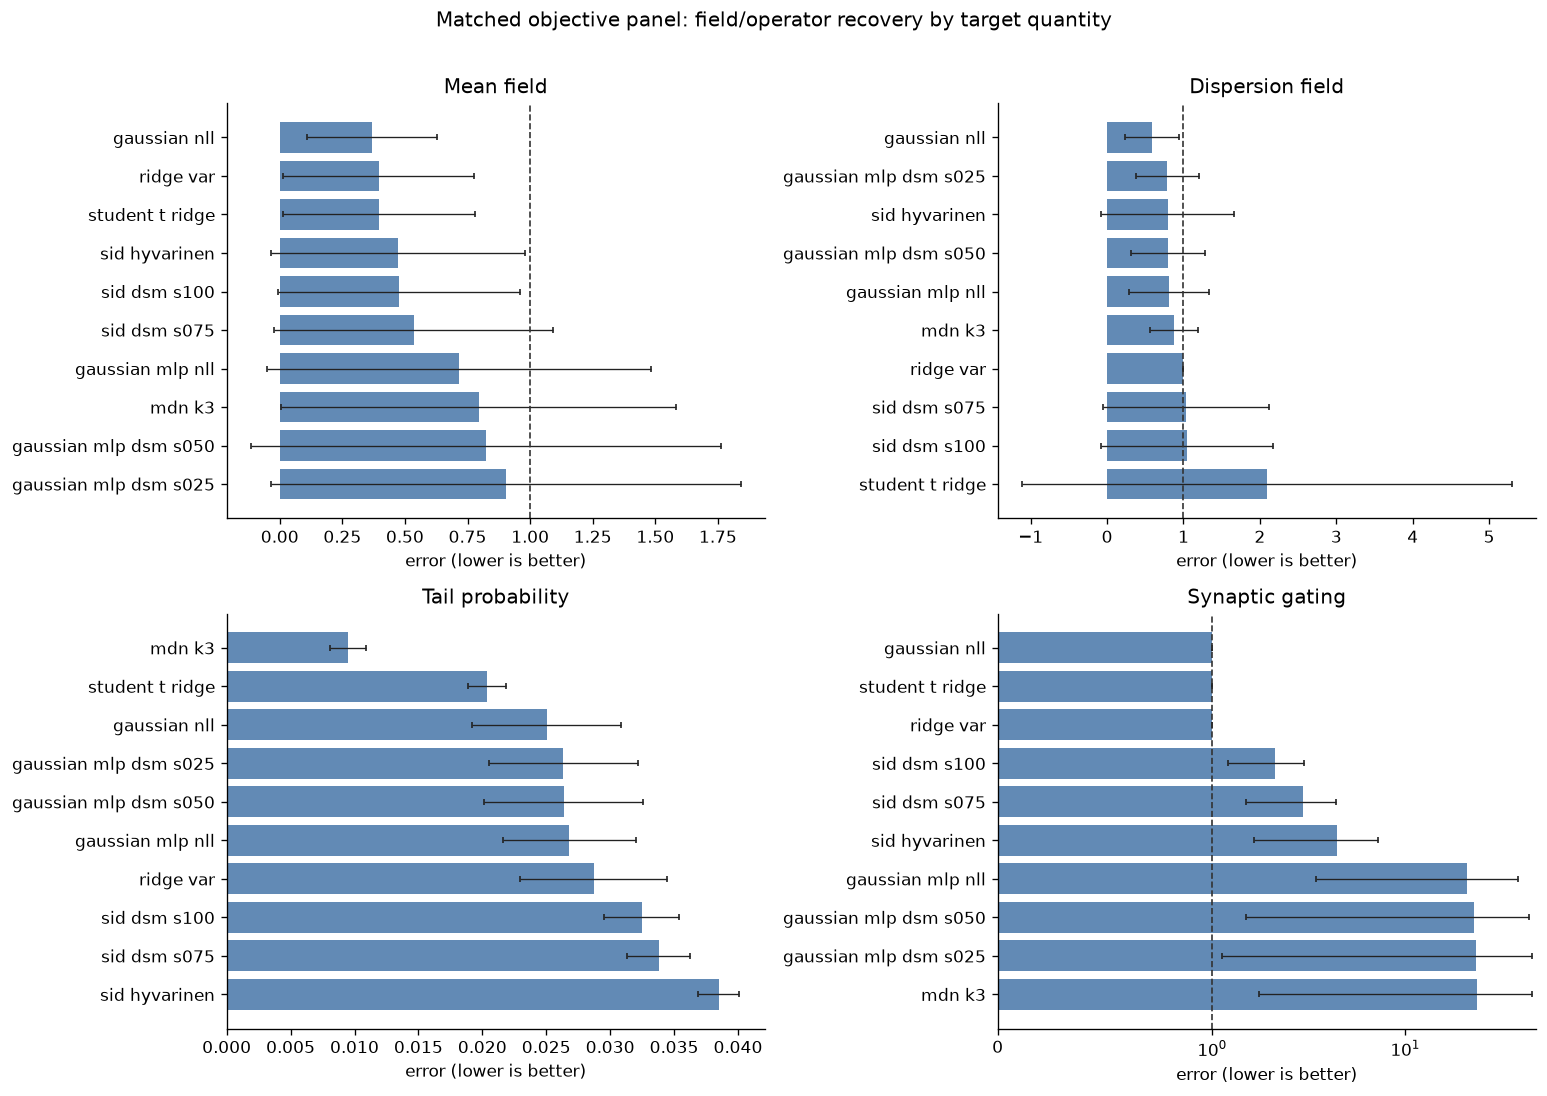
\includegraphics[width=0.93\linewidth]{../../analysis/synthetic_methods_adjudication/objective_parity.png}
  \caption{Matched objective comparison. Methods should be read by estimand: held-out law quality, mean-field recovery, and dispersion-field recovery are different tasks.}
  \label{fig:objective}
\end{figure}

For the physical additive-mean field in the new matched panel:

\begin{center}
\begin{tabular}{@{}lr@{}}
\toprule
Method & Mean-field \(\nise\) \\
\midrule
Penalized Gaussian NLL & \textbf{0.369} \\
Ridge Gaussian & 0.395 \\
Student-\(t\) ridge & 0.395 \\
Quadratic Hyv\"arinen SID & 0.473 \\
Quadratic DSM SID & 0.475--0.535 \\
Neural Gaussian NLL & 0.716 \\
MDN & 0.794 \\
Neural Gaussian DSM & 0.824--0.902 \\
\bottomrule
\end{tabular}
\end{center}

An earlier mechanism panel was even more favorable to classical dynamics: SINDy scored 0.194, sparse transition 0.201, Gaussian NLL 0.246, and Hyv\"arinen SID 0.268. The exact values differ across panels, but the ordering is consistent.

For the physical log-variance field:

\begin{center}
\begin{tabular}{@{}lr@{}}
\toprule
Method & Dispersion-field \(\nise\) \\
\midrule
Penalized Gaussian NLL & \textbf{0.586} \\
Neural Gaussian DSM, \(\sigma=.25\) & 0.789 \\
Quadratic Hyv\"arinen SID & 0.791 \\
Neural Gaussian DSM, \(\sigma=.50\) & 0.794 \\
Neural Gaussian NLL & 0.809 \\
MDN & 0.872 \\
Zero/constant-variance ridge & 1.000 \\
Quadratic DSM SID & 1.037--1.048 \\
Student-\(t\) ridge & 2.091 \\
\bottomrule
\end{tabular}
\end{center}

Neural DSM modestly improves over neural NLL within the same broad Gaussian architecture, so denoising may be a useful derivative regularizer. It does not beat the strictly parameterized Gaussian likelihood. This is evidence for a regularization effect, not a general score-objective advantage.

On the matched-tail law, representational flexibility matters:

\begin{center}
\begin{tabular}{@{}lrr@{}}
\toprule
Method & Held-out NLL & Tail-probability RMSE \\
\midrule
MDN, \(K=3\) & \textbf{-0.614} & \textbf{0.0095} \\
Student-\(t\) ridge & -0.530 & 0.0204 \\
Gaussian NLL & -0.288 & 0.0250 \\
Neural Gaussian DSM & -0.280 to -0.283 & 0.0263--0.0264 \\
Quadratic DSM SID & about -0.283 & 0.0325--0.0338 \\
Quadratic Hyv\"arinen SID & 9.18 & 0.0385 \\
\bottomrule
\end{tabular}
\end{center}

Yet the MDN's physical shape-tail derivative has \(\nise=2.02\), worse than the zero derivative. Predicting a tail probability and estimating its derivative with respect to a modulator are distinct problems.

\subsection{Synaptic gating: no current winner}

All nonzero learned readouts are worse than the zero field:

\begin{center}
\begin{tabular}{@{}lr@{}}
\toprule
Method & Total gating-field \(\nise\) \\
\midrule
Gaussian NLL / ridge / Student-\(t\), emit zero & \textbf{1.000} \\
Quadratic DSM SID & 2.10--2.95 \\
Quadratic Hyv\"arinen SID & 4.42 \\
Neural NLL / DSM / MDN & 20.97--23.40 \\
\bottomrule
\end{tabular}
\end{center}

The trajectories may contain gating, but the present fitted-law readout does not identify its mixed derivative reliably. More hyperparameter search over the same target is unlikely to change the conclusion. The next experiment must first show oracle identification from paired controlled laws or an explicitly gated transition model.

\subsection{History tangents and finite contrasts}

The infinitesimal point-history sweep completed 96 of 96 fits, passed fixed-batch overfit checks, and reproduced under exact replay. Nevertheless, six derivative-readiness gates failed. G1 location tangents reached NRMSE 0.589--0.719, while the best G2 covariance and G3 skew tangents were 1.068 and 1.167. The failure is therefore not explained by gross optimization failure.

\begin{figure}[t]
  \centering
  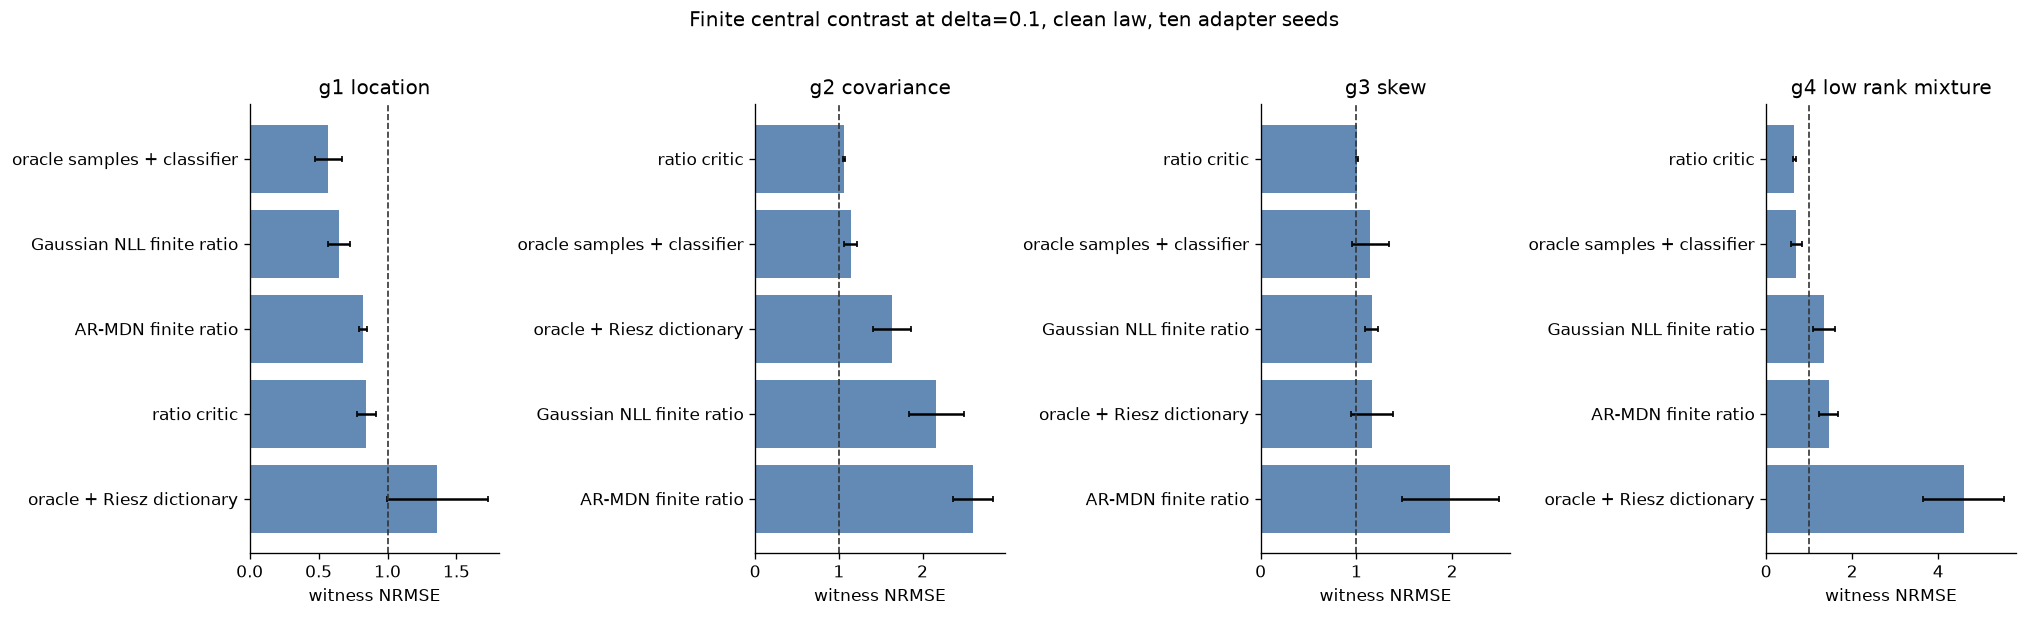
\includegraphics[width=0.98\linewidth]{../../analysis/synthetic_methods_adjudication/finite_contrast_ten_seed.png}
  \caption{Finite-contrast witness NRMSE across ten adapter/evaluation seeds at the main perturbation scale. The dashed reference at 1 is the zero-witness baseline.}
  \label{fig:finite}
\end{figure}

At clean \(\delta=0.1\), the ten-seed finite-contrast panel gives:

\begin{center}
\begin{tabularx}{0.96\linewidth}{@{}lXrX@{}}
\toprule
Generator & Best practically relevant route & Mean NRMSE & Verdict \\
\midrule
G1 location & Direct signed classifier / Gaussian finite ratio & about 0.61--0.65 & Useful; beats zero clearly \\
G2 covariance-only & Ratio critic & 1.057 & No recovery \\
G3 skew-only & Ratio critic & 1.008 & No recovery \\
G4 low-rank mixture & Ratio critic & \textbf{0.656} & Useful; beats zero clearly \\
\bottomrule
\end{tabularx}
\end{center}

The oracle infinitesimal tangent has negligible Taylor mismatch at this \(\delta\) for G2 and G3, but the oracle-sample classifier is still roughly 1.14 NRMSE. Consequently, the primary bottleneck is adapter geometry, response features, calibration, or signal-to-noise---not the learned diffusion generator. The current signed Riesz dictionary should not be scaled until an oracle redesign beats zero.

\subsection{SBTG localization}

The frozen SBTG panel shows joint-score cross-moment average-precision excess of roughly 0.15--0.39 for mean-like support. Similar values occur across additive, dispersion, and synaptic mechanisms, so the statistic is not mechanism-specific. Log-variance localization is only 0.06--0.10, and squared-score-covariance localization is roughly 0.00--0.05. Linear SBTG is often as good as or better than feature-bilinear variants.

The defensible conclusion is that SBTG can remain a reduced-form nonlinear screening/localization route. It has not established recovery of physical dispersion, gating, or a causal graph.

\subsection{Classical graph baselines and hidden confounding}

\begin{figure}[t]
  \centering
  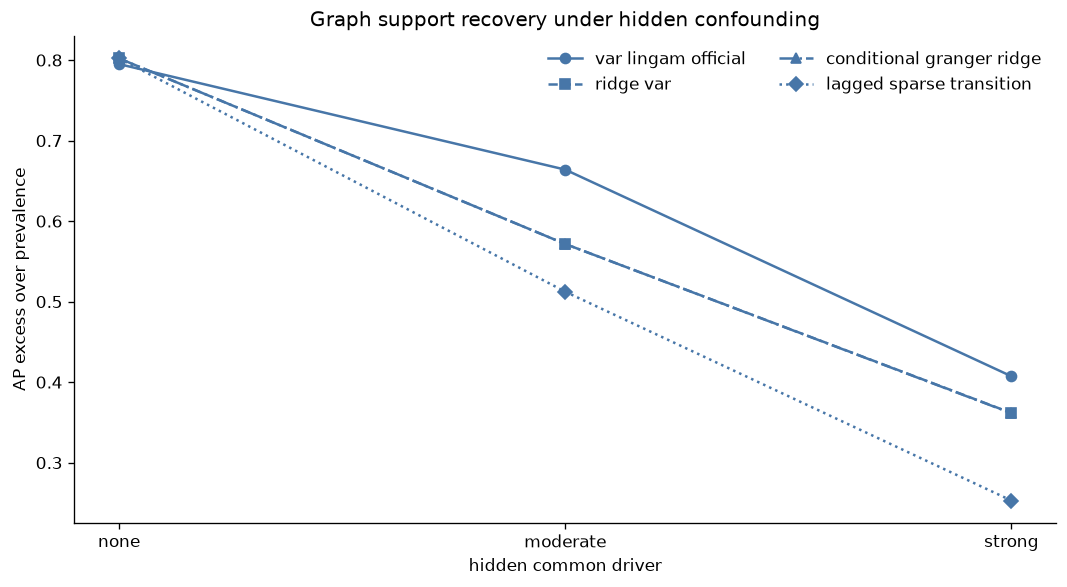
\includegraphics[width=0.74\linewidth]{../../analysis/synthetic_methods_adjudication/graph_hidden_confounding.png}
  \caption{Graph-support average-precision excess under causal sufficiency and strong hidden common drive. Every observational method degrades.}
  \label{fig:graph}
\end{figure}

Under causal sufficiency, classical transition methods reach about 0.80 AP excess. Under a strong hidden common driver, VAR-LiNGAM scores 0.407, ridge VAR 0.362, conditional Granger 0.361, PCMCI 0.338, sparse transition 0.253, and marginal lagged correlation 0.106. These are mandatory comparators. Even the best result is observational support recovery under a violated or stressed assumption, not identification of a latent causal mechanism.

\subsection{Changepoints}

With 199 matched-null calibration trajectories and 100 independent evaluation trajectories per condition:

\begin{itemize}
  \item the mean CUSUM detects and localizes 100/100 high-signal mean changes;
  \item the residual tail-shape probe detects and localizes 100/100 exactly mean/variance-matched tail changes;
  \item the residual variance probe calls 100/100 dispersion changes but localizes only 41/100;
  \item that variance probe also calls 95\% of mean changes and 99\% of matched-tail changes, so it is a broad residual-instability alarm rather than a dispersion-specific detector;
  \item independent-null false-positive rates are 2\% for mean, 4\% for conditional rule and variance, 3\% for tail, 9\% for MMD, and 11\% for energy distance.
\end{itemize}

Mean and tail provide strong matched demonstrations. Dispersion requires nuisance orthogonalization and confusion controls before it can carry a channel-specific label.

\section{Where our approaches have an advantage---and where they do not}

\subsection{Potential advantages}

The unified finite SID approach can be better than existing alternatives for reasons that are conceptual and testable:

\begin{enumerate}
  \item \textbf{Model-agnostic downstream interface.} The same contrast and readout can be applied to a tractable density, an energy model, a diffusion sampler, or an oracle simulator.
  \item \textbf{Exact finite estimand.} Equation~\eqref{eq:finite-witness} avoids pretending that an arbitrarily small derivative is scientifically meaningful or statistically stable.
  \item \textbf{Typed explanation of distributional change.} Unlike a single MMD or energy statistic, the witness can be integrated against declared mean, covariance, interaction, and tail features.
  \item \textbf{Bounded witness construction.} The absolute-coefficient mixture gives a bounded Radon--Nikodym witness, which is attractive for stable estimation and sequential concentration.
  \item \textbf{Multiple overidentifying routes.} Density ratios, classifiers, direct sample moments, and score reconstructions can target the same contrast. Agreement becomes a diagnostic rather than a rhetorical robustness check.
  \item \textbf{Resolution as a scientific parameter.} \(\delta\) specifies the perturbation being studied; \(\sigma\) specifies score corruption. Their effects can be separated and reported.
  \item \textbf{A path from local sensitivities to changes over time.} Once a channel is validated, the same typed statistic can be embedded in offline or online changepoint inference.
\end{enumerate}

\subsection{Costs and failure modes}

Those advantages come with real tradeoffs:

\begin{itemize}
  \item \textbf{Perturbation design:} the direction, magnitude, stencil, and support of \(T_{\delta,v}h\) are part of the estimand and may not be naturally identified from observational histories.
  \item \textbf{Overlap:} finite ratios and classifiers become unstable when \(P_{h_+}\) and \(P_{h_-}\) have little common support; tiny \(\delta\) has the opposite weak-signal problem.
  \item \textbf{Channel conditioning:} covariance, skew, and tail features can have high variance or poor geometry. An omnibus witness may be harder to learn than a direct targeted regression.
  \item \textbf{Derivative instability:} score or density convergence does not automatically imply convergence of derivatives with respect to history.
  \item \textbf{Corruption bias:} DSM learns a smoothed law. Fine changes can be attenuated by the denoising scale.
  \item \textbf{No causality for free:} predictive history dependence can arise from common drive, selection, or omitted state.
  \item \textbf{Computation:} multiple histories, routes, channels, and calibration blocks cost more than a single fitted transition model.
  \item \textbf{Baseline strength:} when the task really is conditional mean estimation under a sparse low-order law, ridge or SINDy is expected to win.
\end{itemize}

\subsection{When diffusion/score methods have a credible hope}

The present negative results do not imply that diffusion-based SID is hopeless. They imply that it needs a home-field experiment. A score/sample backend has a credible advantage when at least one of the following holds:

\begin{itemize}
  \item the conditional law is high-dimensional and multimodal, making normalized likelihood evaluation or integration impractical;
  \item the model is available only as a simulator or sampler;
  \item the scientific target depends on a local portion of response space that a mean/variance model erases;
  \item a shared generative model amortizes many contrasts or channels more efficiently than separately fitting targeted regressions;
  \item sample coupling or common noise can sharply reduce finite-difference variance.
\end{itemize}

To be impactful, the project must demonstrate one of these regimes. Beating a Gaussian likelihood on a near-Gaussian low-dimensional simulator is neither necessary nor likely. Conversely, merely functioning where likelihood is inconvenient is not enough; the method must yield a better estimand, better sample efficiency, or a capability the baseline cannot expose.

\section{Theory agenda}

The framework is conceptually coherent, but several results are needed to turn it into a mature method.

\subsection{Finite-witness stability bounds}

Derive error transfer from predictive laws or ratios to the witness and typed channels. Under overlap bounds and bounded \(\phi\), seek inequalities of the form
\[
  \left|\widehat\Delta_c(\phi)-\Delta_c(\phi)\right|
  \leq C_1\,d(\widehat P,P)+C_2\,\|\widehat W-W\|_{L^2(M)}
  +\text{sampling error},
\]
with explicit dependence on \(\delta\), dimension, and overlap. This would clarify when improving the predictive backend can actually improve the scientific readout.

\subsection{Bias--variance theory for \(\delta\) and \(\sigma\)}

Develop a phase diagram separating:

\begin{itemize}
  \item finite-stencil truncation bias as \(\delta\) grows;
  \item weak contrast and ratio variance as \(\delta\to0\);
  \item posterior smoothing/contraction as denoising noise \(\sigma\) grows;
  \item approximation and discretization error in reverse sampling.
\end{itemize}

The key theoretical question is whether the useful region scales with \(\sigma/\delta\), signal geometry, and intrinsic response dimension.

\subsection{Orthogonal and cross-fitted channel estimation}

Treat \(\Delta_c(\phi)\) as the primary low-dimensional functional and derive Neyman-orthogonal estimators using cross-fitted predictive laws and Riesz representers. This may allow slower nuisance convergence while retaining valid uncertainty for a small set of scientific channels. It is likely more promising for covariance and tail readouts than reconstructing the entire witness with a generic classifier.

\subsection{Reconstructing SID from SBTG}

Formalize the inverse problem in Equation~\eqref{eq:sbtg}. Given an estimate of \(K_v=\nabla_y\ell_v\), recover \(\ell_v\) by a weighted Poisson or Hodge problem with the conditional centering constraint
\[
  \int \ell_v(y;h)p_h(y)\,dy=0.
\]
Prove identifiability and stability under boundary/support assumptions. Compare this reconstruction against direct finite ratios at the oracle level. If the inverse problem is ill-conditioned in the tested regimes, SBTG should remain a localizer rather than the main SID route.

\subsection{Higher-order parity stencils}

Develop first- and second-order signed stencils whose finite witnesses are derived from the correct likelihood-ratio polynomial. A second derivative of a density includes both log-density Hessian and score-product terms; using a log Hessian alone generally targets the wrong signed measure. Establish exact coefficient/reference-mixture constructions and variance-optimal weighting.

\subsection{Route-agreement tests}

When density, classifier, direct-moment, and score routes target the same \(\Delta_c(\phi)\), formulate an overidentification test. Systematic disagreement can diagnose lack of overlap, score non-integrability, density calibration error, or sampler bias. This is potentially a distinctive contribution: the framework creates several estimators of one declared object rather than several incomparable model scores.

\subsection{Mechanism-confusion and nuisance invariance}

For a channel label to be meaningful, derive or enforce orthogonality to nuisance changes. A dispersion statistic should be insensitive to mean shifts; a standardized tail statistic should be insensitive to matched mean and variance changes. Develop residualization, influence-function, or adversarial nuisance-projection schemes and evaluate a full confusion matrix rather than only target power.

\subsection{Sequential inference}

Use bounded finite witnesses to construct blockwise e-values, martingales, or self-normalized scans under temporal dependence. The target result is false-alarm control across repeated monitoring while retaining a typed interpretation. Offline PELT and online BOCPD remain external inference engines; SID should contribute a validated cost or evidence sequence.

\section{The next decisive experiment program}

The next work should be staged. Later phases are conditional on earlier oracle gates; otherwise capacity and compute will obscure identification failures.

\subsection{Observable neuromodulator benchmark ladder}

The attached neuromodulatory hierarchy is useful if it is translated into
observable conditional laws rather than another latent mechanistic state-space
model.  Let $H_t$ contain observed stimulus, neural, behavioral, and
neuromodulator histories, and let $Y_{t+1:t+K}$ be a multichannel future path.
Five nested generator tiers should share histories and random-number streams:

\begin{center}
\begin{tabularx}{\linewidth}{@{}p{0.11\linewidth}p{0.25\linewidth}X@{}}
\toprule
Tier & Declared change & Construction and exact negative controls \\
\midrule
O1 & mean/gain & nonlinear saturating temporal operator with fixed covariance; variance/tail readouts are null \\
O2 & stochastic law & heteroskedastic, Student-$t$, stochastic-release, and mixture residuals matched in mean; location is null \\
O3 & source--target--timescale tensor & sparse multiscale history filters with known low-rank interaction tensor; matched marginal histories and indirect-path controls \\
O4 & spatial field & smooth and localized kernels over uncertain coordinates, with matched global gain and spatially permuted nulls \\
O5 & whole-path topology & G8-type mixture-of-path transports whose occupancy, dwell, or transition law changes while first two conditional moments remain fixed \\
\bottomrule
\end{tabularx}
\end{center}

The nonlinear backbone, residual law, and contrast mechanism must be independently
randomized.  A method should not receive the basis or architecture used to
generate the law.  Recommended primary sizes are 32/96/256 observed channels,
history lengths 16/64, future horizons 8/32, and intrinsic contrast ranks
2/8/16, with at least 20 independent system seeds for any confirmatory claim.
Every tier exposes exact conditional samples, paired latent randomness, and an
exact density or high-precision oracle ratio where tractable.

Process noise and measurement noise are separate axes.  Process axes include
release randomness, heavy-tailed innovations, history-dependent scale, shared
drive, and temporal/spatial correlation.  Observation axes include independent
noise at 0/0.1/0.25/0.5/1 signal SD, calcium-kernel misspecification at
0/10/25/50\%, downsampling by 1/2/4/8, random and structured missing channels at
0/25/50/75\%, shared artifacts, spatial-coordinate error, and intervention-time
jitter.  Single-axis sweeps establish attribution; a frozen composite stress
condition tests robustness.  Training-support interpolation and extrapolation
are reported separately.

The seven scientific endpoints are predictive-law/calibration quality,
perturbation fidelity, gain, variability/covariance, source--target influence
stability, temporal/spatial kernel recovery, and path-transition/dwell effects.
For each endpoint the direct sufficient-statistic regression or empirical paired
contrast is mandatory; a calibrated finite classifier, kernel/MMD or energy
two-sample method, appropriate normalized density, and diffusion/flow backend
receive the same sample and tuning budget.  This design tests whether a shared
generative backend earns its complexity under misspecification, rather than only
whether it can rediscover its own simulator.

\subsection{Phase 0: oracle adapter tournament}

\textbf{Goal.} Determine whether each scientific channel is recoverable from perfect access to the relevant conditional laws before training any flexible predictive model.

\textbf{Data-generating families.}

\begin{itemize}
  \item G1: pure location change;
  \item G2: covariance-only rotation/scale change with fixed mean;
  \item G3: skew-only change with matched mean and covariance;
  \item G4: low-rank mixture interaction;
  \item G8: whole-path topology with exact first/second-moment shadow;
  \item mechanistic fields: additive mean, stochastic dispersion, matched tail, synaptic gating, and correlation-only changes.
\end{itemize}

\textbf{Oracle interfaces.} Exact log density and ratio where available; exact score; independent conditional samples; paired/common-random-number samples; exact moments; exact infinitesimal tangent.

\textbf{Adapters.}

\begin{itemize}
  \item exact finite ratio and direct log-ratio transformation;
  \item calibrated signed logistic classifier;
  \item KLIEP and uLSIF;
  \item polynomial/Hermite, kernel, and learned feature classifiers;
  \item channel-targeted Riesz estimators with cross-fitting;
  \item score-difference plus weighted Poisson/Hodge reconstruction;
  \item mixed SBTG operator plus the same reconstruction;
  \item direct paired-sample channel difference.
\end{itemize}

\textbf{Design.} At least 20 independent generator seeds, with separate data, adapter, and evaluation seeds. Sweep sample size, dimension, \(\delta\), overlap, and signal strength. The main perturbation scale is fixed before inspecting hard-channel results; other scales are sensitivity analyses.

\textbf{Primary metrics.} Witness NRMSE and channel nISE against the zero baseline of 1, with confidence intervals over generator seeds. Secondary metrics are calibration, centering, route disagreement, runtime, and effective sample size.

\textbf{Gate.} A channel advances only if at least one practical oracle adapter has an upper 95\% confidence bound below 1 and the intended channel is distinguishable from nuisance alternatives. G2/G3 currently fail this gate.

\subsection{Phase 1: backend \(\times\) adapter \(\times\) channel factorial}

\textbf{Goal.} Separate predictive-model error from adapter error and determine whether a shared flexible backend helps across multiple channels.

\begin{center}
\begin{tabularx}{\linewidth}{@{}p{0.19\linewidth}X@{}}
\toprule
Axis & Levels \\
\midrule
Backend & Oracle; ridge Gaussian; heteroskedastic Gaussian NLL; Student-\(t\); MDN; \SIDQ-Hyv\"arinen; \SIDQ-DSM; conditional score/diffusion; joint-score SBTG \\
Adapter & Direct density ratio; signed classifier; direct sample channels; Riesz; score/Hodge; mixed SBTG/Hodge \\
Channel & Mean; variance; covariance; low-rank interaction; skew; tail; local occupancy \\
Regime & Correct specification; heavy tails; mixtures; response coupling; high dimension; sample-only access \\
\bottomrule
\end{tabularx}
\end{center}

Every cell is evaluated on the same common estimand. Native NLL or DSM loss is reported only as a backend diagnostic. Exact seed intersections and identical train/validation/evaluation histories are required.

\textbf{Success criterion for diffusion.} A diffusion/score backend must either (i) beat the best feasible normalized backend on a common channel with uncertainty, or (ii) solve a sample-only/intractable-density task where the normalized comparator genuinely cannot expose the estimand, while beating direct empirical and generic two-sample baselines.

\subsection{Phase 2: scaling and stress map}

\textbf{Goal.} Find the regime, if any, where the unified approach has a real advantage.

Sweep:

\begin{itemize}
  \item sample size and effective dependent-block count;
  \item response dimension, history length, and intrinsic contrast rank;
  \item perturbation \(\delta\) and denoising scale \(\sigma\);
  \item observation noise, multimodality, tail weight, and support overlap;
  \item model misspecification and hidden common drive;
  \item number of requested channels/contrasts, to test amortization.
\end{itemize}

Report phase diagrams, not only aggregate ranks. The important question is where each method crosses NRMSE 1, how quickly it improves with data, and whether sharing a backend across many contrasts changes total cost.

\subsection{Phase 3: mechanism-confusion battery}

For every claimed channel, construct matched nuisances:

\begin{center}
\begin{tabular}{@{}lll@{}}
\toprule
Claimed channel & Positive condition & Mandatory negative/confusion conditions \\
\midrule
Mean & mean shift & variance, skew, tail, correlation changes \\
Dispersion & variance/scale change & mean, matched-tail, mixture-weight changes \\
Tail/shape & tail change matched in mean/variance & mean, variance, outlier contamination \\
Interaction & low-rank coupling change & marginal mean/variance changes \\
Graph/localization & edge-specific conditional change & common drive, indirect path, autocorrelation \\
\bottomrule
\end{tabular}
\end{center}

Report a confusion matrix of call rates and localization, not only target AUROC or AP.

\subsection{Phase 4: changepoints only for validated channels}

Carry forward only Phase 0--3 winners. Compare:

\begin{itemize}
  \item channel-specific CUSUM/GLR and PELT costs;
  \item MMD and energy-distance scans;
  \item BOCPD for online inference;
  \item bounded-witness e-value or martingale scans, if theory is ready.
\end{itemize}

Use independent matched-null calibration, independent evaluation, block resampling for dependence, and report false-positive rate, detection power, delay/detection-within-window, localization error, and mechanism confusion. Do not tune thresholds on the evaluation trajectories.

\subsection{Phase 5: long-horizon and pathwise extension}

Only after one-step typed contrasts are reliable, test block or rollout laws \(P(Y_{t+1:t+K}\mid H_t=h)\). Compare recursive and direct multi-horizon densities, conditional samplers, and paired pathwise contrasts. Vary horizon and coupling. The purpose is to learn whether finite SID effects compose or decay across time, not to introduce a separate latent mechanistic model.

\subsection{Preregistered decision rules}

\begin{enumerate}
  \item No learned-backend experiment for a channel whose practical oracle adapter fails the zero baseline.
  \item No downstream changepoint claim for a channel that fails static mechanism-confusion gates.
  \item No winner based only on native loss; all winners must beat baselines on a common population estimand.
  \item Independent generator, data, model-initialization, adapter, and evaluation seeds; exact seed intersections for pairwise comparisons.
  \item A simple zero/no-effect estimator is always included for normalized derivative metrics.
  \item One primary perturbation \(\delta\), corruption schedule, and metric per claim are fixed before evaluation.
  \item Report uncertainty over generator seeds, failure counts, calibration, compute, and route agreement.
  \item Preserve ridge, Gaussian/Student-\(t\) likelihood, MDN, SINDy, Granger/PCMCI/VAR-LiNGAM, MMD, energy, and appropriate changepoint baselines wherever their subproblem applies.
\end{enumerate}

\section{Research priorities and stop/go decisions}

\begin{center}
\begin{tabularx}{\linewidth}{@{}p{0.18\linewidth}p{0.15\linewidth}X X@{}}
\toprule
Direction & Priority & Why & Stop/go criterion \\
\midrule
Finite typed SID & Highest & Most coherent generalization; real G1/G4 wins; model-agnostic & Continue if redesigned oracle G2 or G3 adapter beats zero, or if robust G1/G4 scaling advantage appears \\
Targeted Riesz/orthogonal channels & High & Directly addresses hard covariance/tail functionals and uncertainty & Continue only after oracle cross-fitted estimator is stable and beats direct moment baselines \\
Diffusion as backend & Conditional/high & Needed for sample-only/high-dimensional laws, not low-dimensional Gaussian tasks & Continue if it wins a home-field task or enables a unique validated estimand \\
SBTG-to-SID reconstruction & Medium & Theoretically connects existing ideas and may yield local structure & Continue if oracle \(K_v\to\ell_v\) reconstruction is stable; otherwise retain as screen \\
Channel-specific changepoints & Medium after static gates & Strong mean/tail results; practical downstream use & Advance only validated channels with matched-null and confusion control \\
More \SIDQ sweeps & Low & Current objective parity is decisive on tested parametric tasks & Resume only for a new intractably normalized model or theory-motivated estimator \\
Generic gating mixed derivative & Stop/redesign & Every learned readout loses to zero & Require controlled paired identification or explicit gated parameterization first \\
\bottomrule
\end{tabularx}
\end{center}

\subsection{What would count as an impactful result?}

At least one of the following should be demonstrated:

\begin{itemize}
  \item a high-dimensional non-Gaussian conditional law where flexible-backend \FiniteSID beats feasible likelihood, direct moment regression, and generic two-sample methods on a common typed sensitivity;
  \item a sample-only setting where the framework reliably identifies a localized channel that density-based baselines cannot compute and direct empirical differences cannot estimate efficiently;
  \item a multi-contrast amortization result where one predictive generator plus SID adapters is substantially more accurate or efficient than separately trained targeted models;
  \item a calibrated changepoint system that both detects and correctly labels mean/dispersion/tail/interaction changes with controlled confusion under dependence;
  \item a theorem and experiment showing stable recovery of a centered SID witness from the SBTG mixed operator in a nontrivial class.
\end{itemize}

Without one of these, the framework may remain a useful organizational language but not yet a competitive method.

\section{Recommended paper-level narrative}

A future external paper should not claim that score matching generally outperforms likelihood or that a joint score reveals a causal mechanism. A defensible narrative is:

\begin{enumerate}
  \item Define predictive-law sensitivity through exact finite signed contrasts and typed channel functionals.
  \item Show that normalized densities, classifiers, scores, and samplers are interchangeable computational interfaces to the same estimand.
  \item Establish boundedness, stability, and uncertainty results for the finite witness and its channel readouts.
  \item Demonstrate oracle adapter validity, then learned-backend performance, in regimes where direct mean/variance models are insufficient.
  \item Use SBTG as a related gradient representation and changepoints as a downstream inference application.
  \item Be explicit that causal or mechanistic interpretations require extra assumptions or controlled perturbations.
\end{enumerate}

The strongest conceptual contribution is not a new loss. It is a typed, support-aware interface between predictive generative models and scientifically interpretable distributional sensitivities, together with tests that determine whether the interface is valid.

% Empirical section updated from frozen July 13 artifacts.
\section{Frozen July 13 empirical adjudication}
\label{sec:stable-results}

\begin{takeaway}
Proper full-law fit is not sufficient for the hardest new SID target.  Flexible
autoregressive and flow densities learn G8's static multimodal geometry extremely
well by held-out likelihood, but retain only 3--19\% of the held-out information
about its history-controlled mode weights and their samplers recover at most about
10\% of the corrected fourth-order effect.  A classifier-guided midpoint generator
raises EDM's median effect slope from 0.010 to 0.398 but remains badly attenuated,
and explicit endpoint experts reach only 0.336.  These interventions separate
missing global mass from missing fourth-order generator geometry.  In contrast, a balanced finite
classifier trained on the declared perturbation reaches Bayes AUC and 1--3\%
typed-effect error.  Across the wider suite, direct ratios are the most reliable
clean tangent route, while diffusion's accurate noisy response score frequently
fails to transfer to an accurate history tangent.  The data therefore isolate an
objective/estimand mismatch, not simply insufficient signal or an unstable sampler.
\end{takeaway}

\subsection{Frozen design and validation}

The core run crossed eight exact generators, all applicable models, two generator
seeds, two data seeds, and two model seeds.  All 784 expected cells completed; all
784 case records were valid; there were zero case failures and zero metric
failures.  The run used 8,000 training examples, a fixed 1,600-case validation
set, 512 test cases, one CPU thread, and one job at a time.  The eight crossed
cells per generator--model pair measure data and initialization variability, but
there are only two independent generated systems.  Consequently all intervals in
this subsection are developmental paired-bootstrap summaries, not confirmatory
system-level inference.

The evaluation contract keeps five endpoints distinct:
\begin{enumerate}
  \item fair energy score for conditional samples;
  \item NLL only for models with an exact normalized density;
  \item clean history-tangent NRMSE for direct normalized or ratio routes;
  \item noisy response-score NRMSE at standardized corruption $0.12$;
  \item noisy history-tangent NRMSE for diffusion, separated by its centering
  route.
\end{enumerate}
The zero-tangent estimator has NRMSE one.  The frozen bounded-energy numerical
rows are retained for audit but excluded from the primary fair-energy ranking
because that run used dependent finite-pool SIR.  The implementation has since
been replaced by exact i.i.d. rejection sampling with proposal caps and acceptance
diagnostics; this repairs future evaluation but does not retroactively change the
frozen table.

\subsection{Predictive-law fit: real flexibility gains, but metric-dependent}

Table~\ref{tab:law-winners} gives the best eligible route under the two common law
metrics.  Energy values are mean paired percentage changes from Gaussian NLL;
NLL values are paired nats per response vector.  Negative is better.

\begin{center}
\begin{tabularx}{\linewidth}{@{}l X r X r@{}}
\toprule
Law & Best fair-energy route & Change & Best exact-density route & NLL change \\
\midrule
G1 Gaussian sanity & Gaussian-anchored EDM & $-0.41\%$ & autoregressive MDN & $-0.118$ \\
G2 covariance & autoregressive MDN & $-0.66\%$ & autoregressive MDN & $-0.227$ \\
G3 matched skew & autoregressive MDN & $-0.44\%$ & autoregressive MDN & $-0.665$ \\
G4 separated modes & autoregressive MDN & $-2.25\%$ & autoregressive MDN & $-2.556$ \\
G5 near manifold & autoregressive Transformer & $-4.98\%$ & autoregressive Transformer & $-24.336$ \\
G6 rough history & Gaussian NLL & $0.00\%$ & Gaussian NLL & $0.000$ \\
G7 concentrated support & flow matching & $-1.18\%$ & autoregressive MDN & $-1.228$ \\
G8 functional shape & affine flow & $-1.89\%$ & autoregressive Transformer & $-18.343$ \\
\bottomrule
\end{tabularx}
\captionof{table}{Best eligible law-fit routes in the frozen core panel.}
\label{tab:law-winners}
\end{center}

\begin{figure}[ht]
\centering
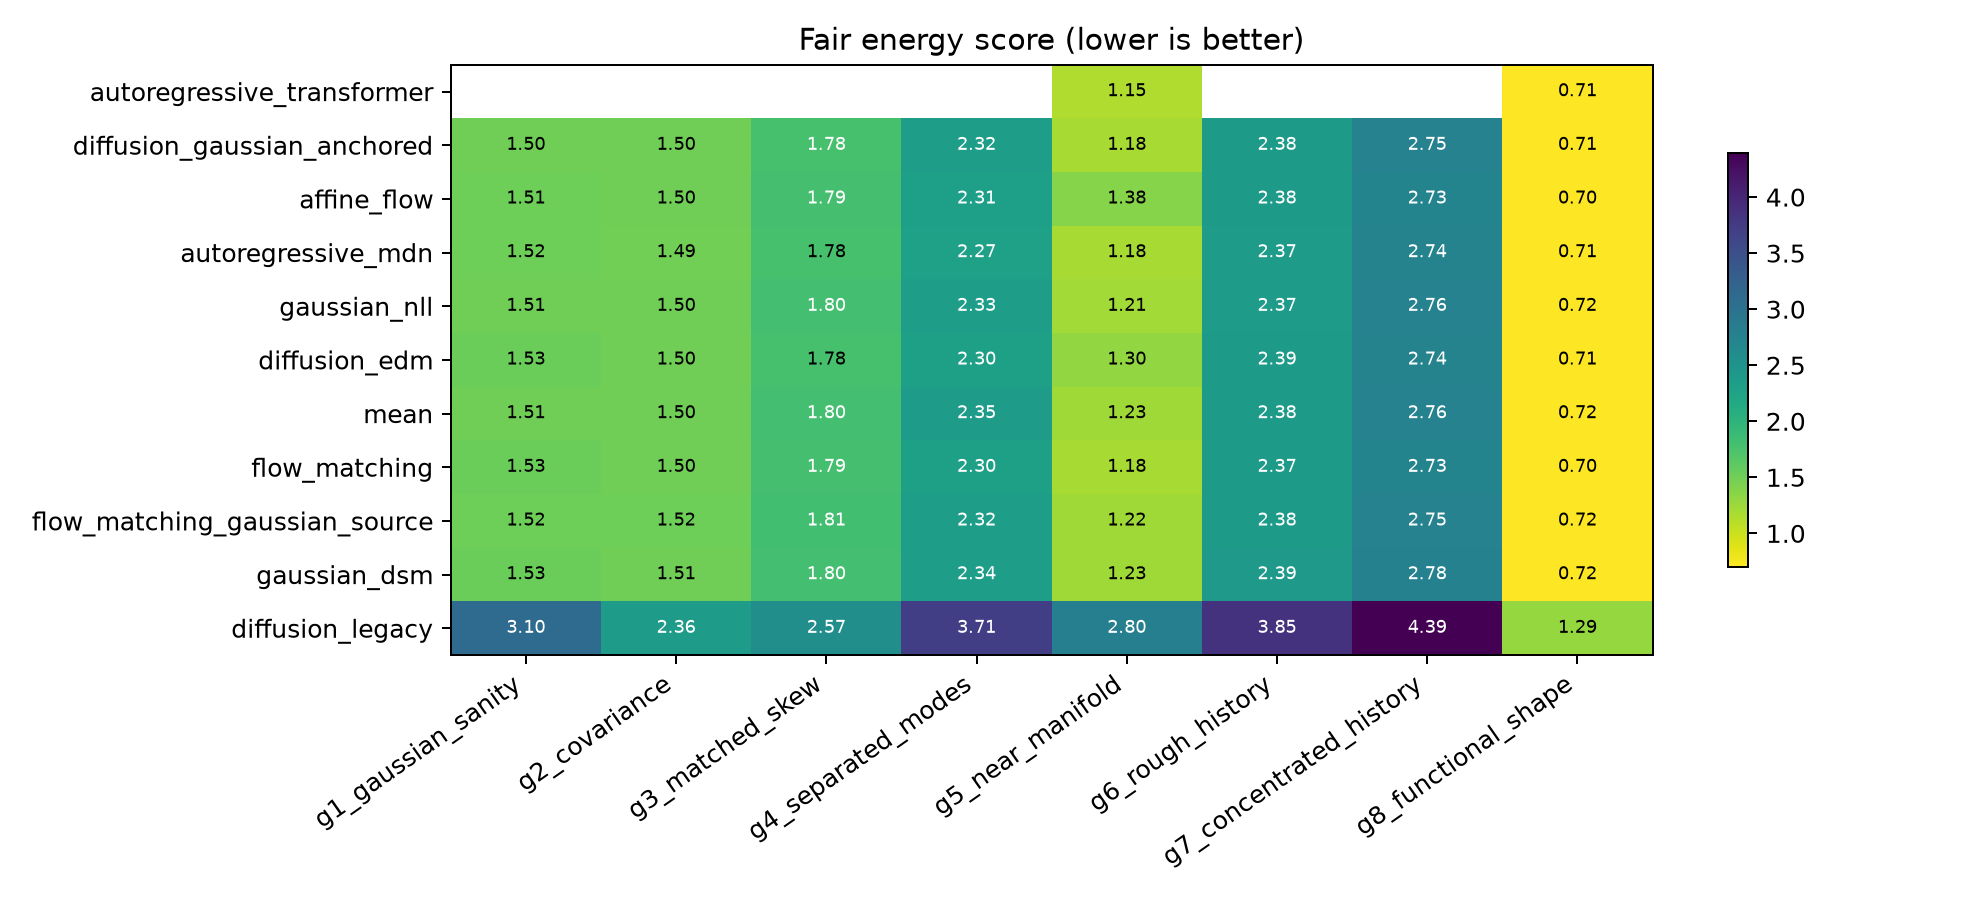
\includegraphics[width=\linewidth]{../../analysis/stable_sid_adjudication_2026-07-13-v2/core_energy_score.png}
\caption{Frozen fair-energy medians.  The bounded-energy row is excluded because
that run's SIR sampler did not provide i.i.d. draws.  Absolute scores should be
compared within a generator, not across response dimensions.}
\label{fig:stable-energy}
\end{figure}

Three conclusions are important.  First, the flexible normalized models clearly
learn non-Gaussian structure: relative to Gaussian, paired NLL improves in every
cell by about 2.56 nats on G4, 24.34 on G5, and 18.34 on G8 for the winning
models.  Second, fair energy sees only small improvements on G4/G7/G8 and can
therefore understate the value of fitting mode topology.  Third, likelihood and
sample geometry can disagree: on G5 the affine flow improves NLL by 23.24 nats
but makes energy score 14.0\% worse.  Neither metric alone is a sufficient SID
gate.

The stabilized EDM sampler is not a universal law winner.  Relative to Gaussian
its mean paired energy changes are $-1.78\%$ on G4, $-0.93\%$ on G7, and
$-1.42\%$ on G8, but $+6.03\%$ on G5 and $+1.37\%$ on G1.  Gaussian anchoring
repairs much of the G5 loss ($-3.25\%$ versus Gaussian), but the autoregressive
Transformer remains better ($-4.98\%$).  The legacy diffusion sampler is
43--130\% worse than Gaussian across the suite despite often having the best
noisy response-score estimate.  Stabilization therefore repairs generation, not
automatically derivative access.

The exact-rejection reevaluation closes the bounded-energy validity gap.  All 64
frozen checkpoints complete with i.i.d. draws; median acceptance ranges from
0.136 to 0.431, and the largest realized proposal tensor contains 4,092 proposals
under a 4,096 cap.  Exact fair-energy medians for G1--G8 are respectively
1.507, 1.504, 1.775, 2.301, 1.209, 2.382, 2.778, and 0.715.  These are competitive
with Gaussian and flow on several laws, but still trail the strongest flexible
frozen baseline on G4/G5/G7/G8.  More decisively, the exact G8 quartic NRMSE is
1.000 with slope $-0.00008$.  Exact sampling repairs the proper-score contract;
it does not repair the contrast objective.

\subsection{Clean SID: the ratio route wins most often, with sharp failures}

\begin{center}
\begin{tabularx}{\linewidth}{@{}l X r X@{}}
\toprule
Law & Best clean tangent route & Median NRMSE & Validity interpretation \\
\midrule
G1 Gaussian sanity & ratio critic & 0.532 & valid in all eight cells \\
G2 covariance & ratio critic & 0.582 & valid in all eight cells \\
G3 matched skew & ratio critic & 1.456 & no route beats zero \\
G4 separated modes & ratio critic & 0.424 & only reliable route \\
G5 near manifold & ratio critic & 0.585 & Transformer second at 0.881 \\
G6 rough history & ratio critic & 0.658 & all direct routes beat zero \\
G7 concentrated support & ratio critic & 1.604 & no route beats zero \\
G8 functional shape & autoregressive Transformer & 0.529 & ratio critic second at 0.616 \\
\bottomrule
\end{tabularx}
\captionof{table}{Clean history-tangent NRMSE; the zero estimator is one.}
\label{tab:clean-tangent-winners}
\end{center}

\begin{figure}[ht]
\centering
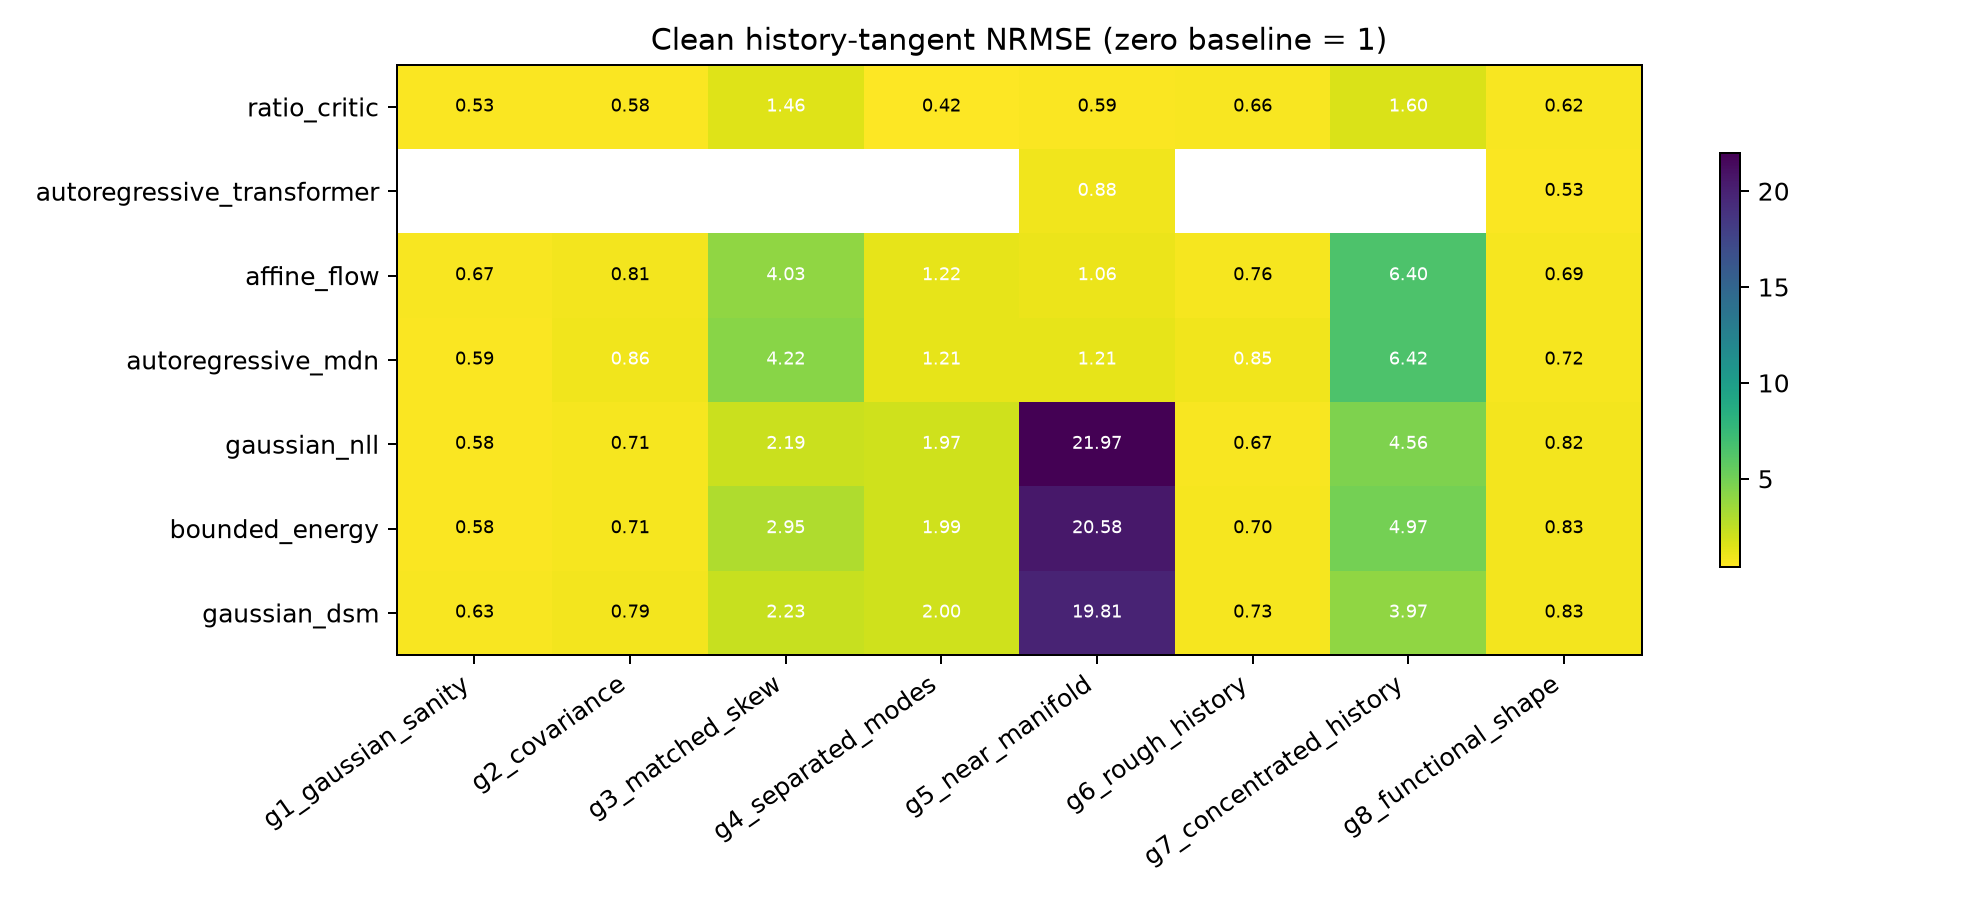
\includegraphics[width=\linewidth]{../../analysis/stable_sid_adjudication_2026-07-13-v2/core_clean_tangent_nrmse.png}
\caption{Clean history-tangent NRMSE with estimand and centering route held fixed.
Values above one lose to the zero-tangent estimator.}
\label{fig:stable-clean-tangent}
\end{figure}

This is the strongest empirical support for the SID-driven framing.  A direct
ratio critic is the clean-tangent winner on six of eight laws and is particularly
strong for separated mode occupancy (0.424) and the near-manifold mixture
(0.585), where the Gaussian tangent is unusable (1.97 and 21.97).  The normalized
Transformer wins G8 (0.529).  However, the ratio route is not a universal cure:
G3 skew and G7 concentrated support remain invalid at 1.456 and 1.604.  On the
one-sided finite log-ratio metric, every existing G8 route is invalid: ratio critic
1.066, Transformer 1.071, affine flow 1.086, and Gaussian 1.134.  Thus the law is
learnable while the declared finite adaptation is not yet reliable.

\subsection{Diffusion: response score and history SID empirically decouple}

The legacy diffusion has the lowest noisy response-score NRMSE on every generator
(0.216--0.753), yet after implementable model-sample centering its history-tangent
NRMSE is invalid on G3, G4, G5, and G7.  The corresponding medians are 2.390,
1.166, 1.125, and 5.852.  EDM and Gaussian-anchored EDM generally have better
samplers but worse mixed-history derivatives; on G8 their model-centered tangent
NRMSEs are 1.246 and 0.850 versus 0.631 for legacy diffusion.  This reverses their
sample-quality ordering.

An independent five-system invalidity replication reaches the same
location-versus-shape conclusion.  Averaging three fixed Transformer coordinate
orders, Transformer/diffusion tangent NRMSE is 0.497/0.751 on G1 location and
0.636/0.745 on G6 rough location, but 1.272/1.480 on G2 covariance,
1.014/3.852 on G3 skew, and 1.065/1.030 on G4 occupancy.  The oracle clean-to-noisy
gap is below 0.018, so small corruption does not explain the failure.  A
data-only history-Hyv\"arinen penalty also failed its frozen G2--G4 gate.  These
replications rule out the explanation that the core result is only one unlucky
initialization or one EDM implementation choice.

In a separate 64-dimensional G5 development system, the converged Transformer
has energy 1.1768, EDM 1.3226 (12.4\% worse), and legacy diffusion 1.7072
(45.1\% worse).  Diffusion generates samples roughly 250 times faster, so it has
a genuine computational advantage but no demonstrated quality advantage in that
system.

\subsection{Finite typed contrasts}

The frozen finite panel uses the exact same source/checkpoint snapshot, three
perturbation scales $\delta\in\{0.05,0.12,0.25\}$, and clean/noisy response laws.
Its complete manifest contains 212,832 valid metric rows, 4,704 diagnostic rows,
eight generators, 14 predictive-source labels, and seven finite routes; no metric
row failed.  The learned cells cross the same two generator, two data, and two
model seeds as the core panel.  One adapter seed is used, so these are exploratory
medians rather than adapter-robust confidence intervals.

At the primary clean scale $\delta=0.12$, the best learned typed-channel routes
are:

\begin{center}
\begin{tabularx}{\linewidth}{@{}l X r X@{}}
\toprule
Law & Best route/source & NRMSE & Interpretation \\
\midrule
G1 location & coupled samples, anchored EDM & 0.327 & clear recovery \\
G2 covariance & coupled samples, flow matching & 0.417 & clear recovery \\
G3 matched skew & signed Riesz, legacy diffusion & 1.003 & no valid route at this scale \\
G4 separated modes & central log ratio, MDN & 0.442 & clear recovery \\
G5 near manifold & central log ratio, ratio critic & 0.492 & clear recovery \\
G6 rough history & coupled samples, flow matching & 0.477 & clear recovery \\
G7 concentrated support & coupled samples, flow matching & 0.656 & useful but variable \\
G8 functional shape & coupled samples, Gaussian-source flow & 0.988 & cubic dictionary is blind \\
\bottomrule
\end{tabularx}
\end{center}

This is more favorable to sampler backends than the infinitesimal-tangent panel.
Direct common-random-number sample moments let flow or stabilized diffusion lead
G1, G2, G6, and G7; normalized or direct ratios lead G4 and G5.  Full-witness
reconstruction remains harder.  The best witness NRMSEs are 0.508 (G1), 0.651
(G2), 0.342 (G4), 0.639 (G5), 0.724 (G6), and 0.698 (G7), while G3 and G8 remain
approximately the zero witness.  The signed Riesz dictionary is generally
unstable and should not advance in its present form.

Perturbation scale is scientifically material.  At $\delta=0.25$, direct EDM
samples recover the G3 typed skew channel at NRMSE 0.660 versus an oracle-sample
Monte Carlo floor of 0.430; at $\delta=0.12$ the same clean route is 1.042.  At
the noisy $\sigma=0.12$ law and $\delta=0.12$, EDM reaches 0.727.  This is a real
home-field hint for stabilized generative sampling, but it does not establish
clean infinitesimal skew recovery: increasing $\delta$ changes the estimand, and
response noising changes the law.  More generally G4--G7 improve as the supported
contrast grows, reinforcing the finite rather than infinitesimal formulation.

The process returned nonzero only after atomically writing the complete artifacts,
when a post-write disk guard measured 3.87 GiB free against a 4.00 GiB floor.  The
manifest status, row counts, finiteness, and hashes were independently verified;
the resource event is retained in the audit rather than relabeled as a scientific
failure.

The G8 conclusion requires the analytically necessary fourth-order motif and exact
frame-occupancy readouts.  The current fixed response dictionary ends at cubic
order and is a predeclared negative-control limitation rather than evidence that
G8 has no signal.

The omitted target is not weak.  For generator seeds 61 and 67, the analytic
quartic constants are $D=8.619$ and $7.583$.  At control zero the exact central
quartic effects are 5.170/4.548 at $\delta=0.05$, 5.162/4.542 at
$\delta=0.12$, and 5.133/4.516 at $\delta=0.25$.  A 25,000-draw-per-side oracle
check at $\delta=0.12$ recovers both effects within 0.78 Monte Carlo standard
errors, while linear and quadratic motif contrasts stay near zero.  Hence a
learned method that misses the corrected quartic channel is missing a strong,
exactly identified higher-order effect; a cubic dictionary simply never asked the
right question.

A corrected frozen-checkpoint sample evaluation then asks that question directly.
It covers 96 records with 12 histories and 512 draws per side for every eligible
model; the oracle uses 2,048.  The oracle quartic NRMSE is 0.117 and its median
effect-calibration slope is 0.984.  Every learned sampler is essentially the zero
effect estimator:
\begin{center}
\begin{tabular}{@{}lrr@{}}
\toprule
Backend & Quartic NRMSE & Effect slope \\
\midrule
autoregressive MDN & 0.946 & 0.060 \\
affine flow & 0.949 & 0.051 \\
EDM & 0.994 & 0.006 \\
autoregressive Transformer & 0.994 & 0.007 \\
ordinary flow matching & 0.999 & 0.001 \\
Gaussian NLL & 1.000 & 0.000 \\
\bottomrule
\end{tabular}
\end{center}
Thus the large G8 likelihood gains come from learning the static multimodal path
geometry, while the backends recover only 0--6\% of its history-controlled
fourth-order effect.  This refines the diagnosis again: the original readout was
blind, and the fitted predictive laws use too little of their capacity for the
history-controlled mass change.  A continuously varying history with one response
per history could have contributed, so a separate factorial tests that hypothesis
directly.

That 48-cell factorial crosses two independent systems, two model seeds, a
balanced binary control, and a fixed-budget paired design with four outcomes per
state/control cell.  Binary randomization improves the strongest slope only to
$9.5\%$; fixed-budget pairing does not rescue it:

\begin{center}
\begin{tabular}{@{}lrr@{}}
\toprule
Backend & Unpaired binary slope & Paired/replicated slope \\
\midrule
autoregressive MDN & 0.095 & 0.082 \\
affine flow & 0.046 & 0.050 \\
autoregressive Transformer & 0.049 & 0.024 \\
EDM & 0.013 & 0.016 \\
flow matching & 0.001 & $-0.001$ \\
Gaussian NLL & 0.000 & 0.000 \\
\bottomrule
\end{tabular}
\end{center}

All 48 fits completed without failure.  The paired lane holds total training
rows at 8,000, so its additional within-state replication trades off against the
number of unique states; it rules out that fixed-budget repair, not every possible
replication regime.  More importantly, the shape control is state-independent in
G8, so persistent attenuation after a large supported $-1$ versus $+1$ contrast
points toward objective/representation allocation rather than local support or a
weak perturbation.

An exact noise-scale audit isolates why denoising is especially vulnerable on
this law.  Across four independent G8 systems and 5,000 exact draws per control
side and system, the clean $+1$ versus $-1$ laws retain median
Jensen--Shannon divergence $0.151$ nats and Bayes AUC $0.770$.  Their response
scores differ by only $3.86\%$ of the score RMS, while the history-tangent RMS is
$0.595$.  Noising initially exposes the inter-frame ambiguity region: relative
response-score separation peaks at $13.56\%$ near $\sigma=0.20$.  But at that
same scale Jensen--Shannon divergence has already fallen to $0.0887$ nats.  By
$\sigma=0.60$, divergence is $0.00195$ nats and history-tangent RMS is $0.0670$.
Thus the DSM signal has a narrow intermediate-noise window; ordinary averaging
over noise levels is poorly aligned with preservation of the finite SID target.

\begin{figure}[ht]
\centering
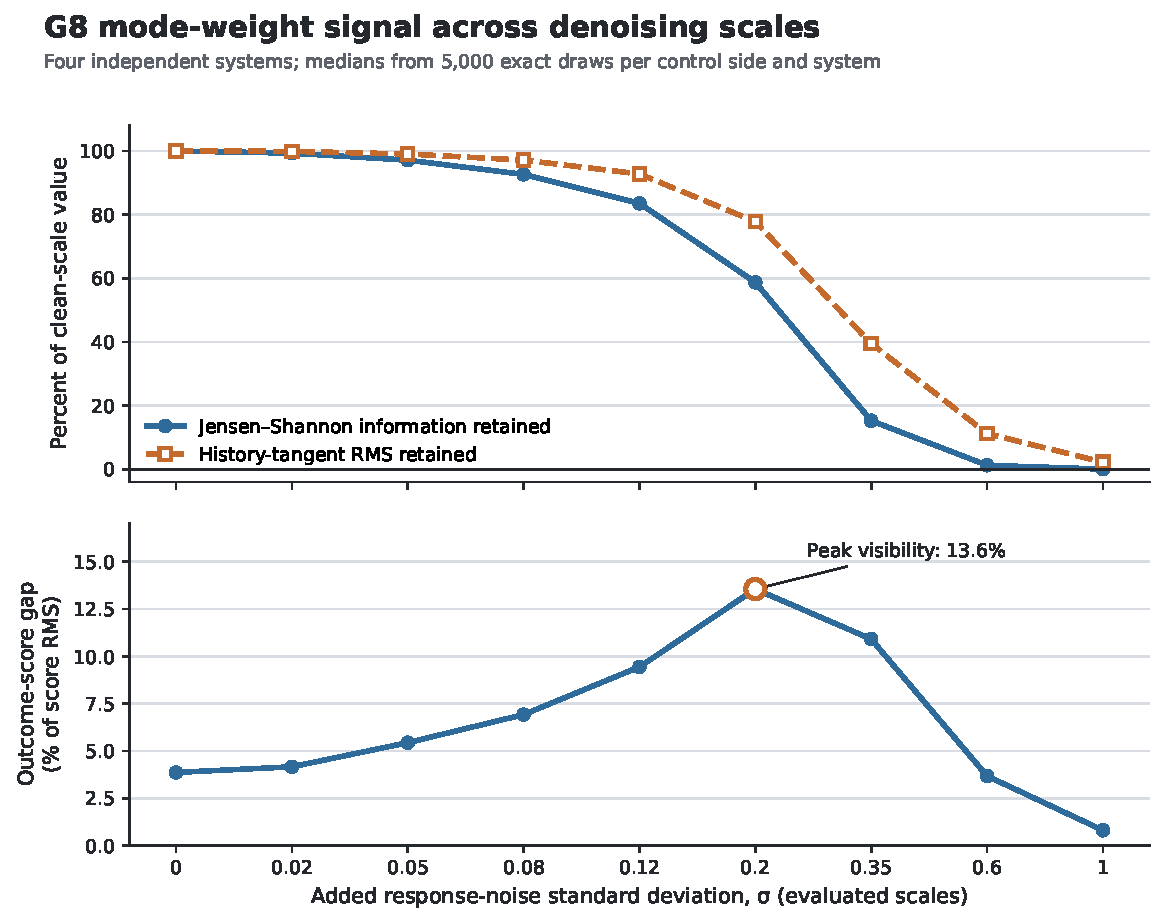
\includegraphics[width=\linewidth]{../../analysis/g8_score_visibility_audit_2026-07-13/g8_score_visibility.pdf}
\caption{Oracle visibility of the G8 mode-weight contrast across denoising
scales.  Top: finite law information and history-tangent magnitude, normalized
to the clean scale.  Bottom: separation between the two conditional outcome
scores relative to their RMS magnitude.  Points are medians over four independent
systems; each system uses 5,000 exact draws per control side.}
\label{fig:g8-score-visibility}
\end{figure}

The contrast itself is nevertheless learnable.  A separate balanced-classification
experiment trains directly on 4,000 responses per control side, tunes on 1,000,
and evaluates on 10,000 held-out responses per side.  It crosses four independent
G8 systems and two data seeds per system.  No classifier receives the control
label as an input.  With equal class priors, its probability estimate is converted
to the exact bounded finite witness $(2\widehat\eta-1)/\delta$ and then integrated
against the quartic readout.

\begin{center}
\begin{tabular}{@{}lrrr@{}}
\toprule
Estimator & AUC & Witness NRMSE & Median effect error \\
\midrule
Bayes witness & 0.768 & 0.000 & 0.33\% \\
empirical typed difference & --- & --- & 0.70\% \\
MLP on motif coordinates & 0.768 & 0.229 & 1.13\% \\
typed quartic logistic & 0.768 & 0.372 & 1.16\% \\
fourth-order polynomial logistic & 0.768 & 0.346 & 2.24\% \\
MLP on raw path and baseline history & 0.763 & 0.421 & 3.05\% \\
quadratic motif logistic & 0.508 & 1.002 & 99.64\% \\
linear motif logistic & 0.499 & 1.000 & 100.00\% \\
\bottomrule
\end{tabular}
\end{center}

This is the cleanest positive result in the new suite.  The flexible contrast
classifier reaches Bayes AUC and accurately recovers the typed effect; the raw
32-dimensional path model does nearly as well without the oracle motif basis.
Linear and quadratic routes stay at chance and reproduce the exact negative
controls.  Full witness recovery remains harder than one projected functional---the
motif MLP has witness NRMSE 0.229 despite only 1.13\% typed-effect error---which is
direct evidence for typed projection rather than unnecessary reconstruction of
the entire law derivative.

The exact first/second-moment Gaussian shadow supplies the mandatory confusion
control.  Across the same four system seeds and two data seeds, the raw
path/history classifier has median AUC 0.499 (range 0.496--0.505).  Its absolute
projected quartic effect is below 0.16\% of the matched positive G8 effect in every
cell.  Thus neither a low-order mismatch nor accidental inclusion of the control
label explains the positive G8 result.

This panel is developmental, not confirmatory: it has only four independent
systems, uses clean histories, and studies the supported $-1$ versus $+1$
contrast.  The motif and quartic variants use oracle centering/basis information;
the raw path/history MLP is the relevant representation-agnostic comparator.  Its
10,000-draw evaluation is larger than the sampler audit, although plug-in standard
errors projected to 512 draws per side are still only 2.0\% of truth for the
motif MLP and 2.4\% for the raw model.  A final common-budget replication remains
required.

A frozen-generator repair experiment then samples each fitted G8 control-zero
midpoint law and reweights those draws with the same raw path/history classifier.
It crosses two independent systems, two data seeds, two model seeds, and five
generator families.  The exact midpoint law with the learned classifier reaches
median NRMSE 0.125 and slope 0.889; replacing the learned classifier by the Bayes
posterior reaches NRMSE 0.013 and slope 1.001.  Thus the reweighting identity and
Monte Carlo procedure are numerically valid.

\begin{center}
\begin{tabular}{@{}lrrrr@{}}
\toprule
Frozen proposal law & Raw NRMSE & Raw slope & Guided NRMSE & Guided slope \\
\midrule
EDM & 0.991 & 0.010 & 0.602 & 0.398 \\
flow matching & 0.992 & 0.009 & 0.648 & 0.353 \\
affine flow & 0.945 & 0.055 & 0.661 & 0.340 \\
autoregressive MDN & 0.941 & 0.060 & 0.669 & 0.332 \\
autoregressive Transformer & 0.996 & 0.005 & 0.737 & 0.264 \\
\bottomrule
\end{tabular}
\end{center}

All 44 records, including four oracle-midpoint controls, completed successfully.
Median guided effective sample fractions are 0.83--0.84 and classifier
probabilities almost never saturate, so importance degeneracy is not the failure.
Guidance recovers a real fraction of the missing mass effect for every proposal
law, but none approaches the exact-midpoint control.  In the error decomposition
of the main text, the contrast head is useful while the $Q$-versus-$M$ geometry
term remains large.  This rejects both extreme explanations: the generator is not
irrelevant, and a classifier head alone is not a complete generative repair.

An 80-cell endpoint-expert factorial tests the complementary repair: enforce the
global gate first, then fit a separate full-law expert to each supported endpoint.
The total budget remains 8,000 rows (4,000 per expert), the declared control is
removed from expert inputs, and the gate deterministically selects the $-1/+1$
expert.  It crosses four systems, two data seeds, two model seeds, and five
backends; every cell succeeds.

\begin{center}
\begin{tabular}{@{}lrrr@{}}
\toprule
Endpoint expert & Fair energy & Quartic NRMSE & Quartic slope \\
\midrule
EDM & 0.704 & 0.665 & 0.336 \\
affine flow & 0.704 & 0.750 & 0.251 \\
autoregressive MDN & 0.714 & 0.823 & 0.179 \\
flow matching & 0.703 & 0.965 & 0.035 \\
Gaussian NLL & 0.718 & 1.000 & 0.000 \\
\bottomrule
\end{tabular}
\end{center}

Compared with shared balanced-control fits, explicit experts materially improve
EDM (slope 0.013 to 0.336), affine flow (0.046 to 0.251), MDN (0.095 to 0.179),
and flow matching (0.001 to 0.035).  Yet they remain far below the direct finite
classifier.  This is the strongest architectural diagnosis in the suite: weak
conditioning is one failure, while a full-law expert objective that underweights
the fourth-order topology is another.  A normalized gate is necessary here but
not sufficient.

The frozen-anchor stochastic-interpolant factorial supplies a separate transport
control.  It reuses the exact core splits and Gaussian anchors, changes only
$\beta_t=t$ versus $t^2$, fixes diffusion amplitude one, and crosses the same two
systems, two data seeds, and two model seeds on G1 and G8.  All 32 fits succeeded.

\begin{center}
\begin{tabular}{@{}llrrr@{}}
\toprule
Law & Schedule & Fair energy & Typed NRMSE & Typed slope \\
\midrule
G1 Gaussian location & linear & 1.513 & 0.338 & 0.908 \\
G1 Gaussian location & squared & 1.513 & 0.319 & 0.864 \\
G8 fourth-order path & linear & 0.717 & 0.993 & 0.0075 \\
G8 fourth-order path & squared & 0.710 & 0.999 & 0.0007 \\
\bottomrule
\end{tabular}
\end{center}

Typed columns use the G1 finite mean effect and the supported G8 quartic effect at
$\delta=1$.  The 64/128/256-step G8 slopes agree to within about one percentage
point.  Squared $\beta$ improves G8 fair energy but worsens the SID channel, while
both schedules learn a nontrivial G1 mean effect.  This is direct evidence against
the two most convenient optimization explanations: the sampler is stable, and
removing the initial response impulse does not expose the missing mass derivative.

Finally, an exact-density permutation audit removes sampling and quartic-readout
noise.  It measures the held-out log-density gain from supplying the correct
shape control instead of a permuted control.  The oracle gain is median 0.274
nats.  The autoregressive MDN retains 19.4\% of it, affine flow 12.4\%, and the
autoregressive Transformer only 2.9\%; Gaussian NLL and Gaussian DSM retain zero.
Thus the attenuation is already present in the fitted conditional density and is
not created by the sampler or the fourth-order statistic.


\section{Final answer to the strategic questions}

\textbf{Which of our methods works best?}  For estimating one scientifically
declared law change, the best original method is now the direct finite
classifier/ratio version of typed SID.  A ratio critic is the clean-tangent winner
on six of eight laws, and a balanced classifier recovers G8's pure fourth-order
path effect within 1--3\% median error while linear and quadratic baselines recover
none.  For fitting an entire predictive law, the answer is problem-dependent:
Gaussian NLL remains best on its home field, while MDNs and autoregressive
Transformers make large NLL gains on multimodal and near-manifold laws.  Those
proper-law gains do not guarantee conditional sensitivity.  Neither standalone
diffusion/DSM nor flow matching is currently the best SID estimator.

\textbf{Do the non-winners have hope?}  Yes, but only in roles consistent with
what they identify.  Diffusion, stochastic interpolants, and function-space score models have a credible
role as whole-path, within-mode, or sample-only generators.  They do not have a
credible standalone route to history-controlled masses on separated components;
that regime requires a normalized mixture gate, finite classifier, ratio, or
bounded energy head.  Stable Target Field, topology-window noise weighting, EDM
preconditioning, and stochastic interpolants can reduce variance or transport
difficulty, but cannot create the missing component constants.  The completed
interpolant factorial confirms that boundary: squared $\beta$ improves G8 fair
energy but its quartic slope is only 0.0007 at 128 steps, with the same conclusion
at 64/256 steps.  SBTG has hope on
connected, well-conditioned laws as a localizer or as a centered Poisson/Hodge
reconstruction with a proved stability constant.  It should not lead on separated
mode weights.  Covariance and skew channels remain open because their existing
adapters fail even with oracle access.

\textbf{Where are we going?}  Toward a contrast-first hierarchy: (i) direct
finite classifier and projected-moment baselines for every declared readout;
(ii) normalized mixture-of-experts or bounded ratio/energy heads for global mass;
(iii) diffusion, flow, or function-space operators only for residual path geometry
that simpler normalized models cannot fit; and (iv) joint history/future
measurement stress tests only after the clean-law channel passes.  Exact rejection
sampling makes the bounded energy backend valid but does not make it the winner;
post-hoc classifier guidance raises EDM's G8 slope only to 0.40, and explicit
endpoint experts reach 0.34.  The decisive next experiment is a common-budget
mixture-gated, contrast-aligned diffusion/flow versus direct
classifier, MDN, autoregressive likelihood, kernel two-sample, and empirical typed
difference on several independent high-dimensional path laws.  Static validity
and route agreement precede changepoints or real neural interpretation.

\appendix

\section{Reproducibility and evidence map}

This synthesis concerns theory and synthetic data only. Real neural-data performance is intentionally outside scope. The principal local evidence sources are:

\begin{itemize}
  \item \path{SYNTHETIC_METHODS_REPORT_2026-07-12.md}: prior adjudication and exact result summaries;
  \item \path{analysis/synthetic_methods_adjudication_2026-07-12.ipynb}: executed analysis notebook;
  \item \path{analysis/synthetic_methods_adjudication/method_taxonomy.csv}: method inventory;
  \item \path{neuromod_benchmark/configs/objective_adjudication_20260712.yaml}: matched objective configuration;
  \item \path{neuromod_benchmark/outputs/objective_adjudication_20260712/}: 250-case matched objective outputs;
  \item \path{history_tangent_benchmark/results/revised_note_v1_finite_contrast_20260712_seed5004} through \path{seed5013}: ten-seed finite contrast outputs;
  \item \path{neuromod_benchmark/outputs/rethink_suite_20260712_v2/}: 24-neuron E1--E5 run with neural and score-model panel (840 fits);
  \item \path{neuromod_benchmark/outputs/rethink_suite_20260712_n32_fast/}: 32-neuron scale confirmation (672 fits);
  \item \path{neuromod_benchmark/outputs/rethink_suite_20260712_sid_stability/}: 432-fit SID regularization/corruption diagnostic;
  \item \path{neuromod_benchmark/docs/THEORY.md} and \path{neuromod_benchmark/docs/METRIC_CONTRACT.md}: estimands, claim ladder, and metric contract;
  \item \path{tmp/pdfs/SBTG_Revised_Technical_Note_July_2026.txt}: revised predictive-generator and finite-witness theory note.
  \item \path{history_tangent_benchmark/results/stable_sid_core_20260713/}: frozen 784-cell core run;
  \item \path{history_tangent_benchmark/results/stable_sid_finite_20260713/}: complete 212,832-row finite-contrast run and manifest;
  \item \path{analysis/g8_typed_classifier_benchmark_2026-07-13/}: eight-cell direct finite-classifier audit;
  \item \path{analysis/g8_gaussian_shadow_negative_control_2026-07-13/}: eight-cell matched-moment classifier negative control;
  \item \path{analysis/g8_classifier_guided_generator_2026-07-13/}: 44-record frozen-generator guidance experiment;
  \item \path{analysis/g8_endpoint_expert_decomposition_2026-07-13/}: 80-cell contrast-aligned endpoint-expert factorial;
  \item \path{analysis/focused_stochastic_interpolant_2026-07-13/}: 32-fit frozen-anchor schedule and sampler-resolution factorial;
  \item \path{analysis/exact_bounded_energy_reevaluation_2026-07-13/}: 64-checkpoint exact-rejection reevaluation;
  \item \path{analysis/g8_score_visibility_audit_2026-07-13/}, \path{analysis/g8_control_information_audit_2026-07-13/}, and \path{analysis/g8_control_design_factorial_2026-07-13/}: score visibility, exact control information, and control-design audits.
\end{itemize}

Software checks at the time of final synthesis passed 103 history-tangent tests,
including analytic exact-rejection, G8 geometry/readout/shadow, and
stochastic-interpolant protocol tests, with three pre-existing Transformer
warnings.  The prior neuromod benchmark suite passed 247 tests. Passing tests
establishes implementation consistency, not scientific identification; the oracle
and baseline gates in this report are stricter.

\section{Compact claim ladder}

\begin{center}
\begin{tabularx}{\linewidth}{@{}p{0.18\linewidth}X X@{}}
\toprule
Claim type & What is supported & What is not implied \\
\midrule
Predictive law & Held-out conditional distribution fit & Correct derivatives or physical mechanism \\
Finite contrast & Difference between declared supported histories & Infinitesimal effect outside the stencil; causal intervention \\
Typed channel & Change in a declared response feature & Other channels or a unique mechanism \\
Localization/graph & Reduced-form predictive dependence support & Causal edge under hidden confounding \\
Changepoint & Calibrated detection/localization of a statistic change & Mechanism label unless confusion gates pass \\
\bottomrule
\end{tabularx}
\end{center}

\begin{thebibliography}{99}

\bibitem{hyvarinen2005}
A. Hyv\"arinen.
Estimation of non-normalized statistical models by score matching.
\emph{Journal of Machine Learning Research}, 6:695--709, 2005.
\url{https://jmlr.org/papers/v6/hyvarinen05a.html}

\bibitem{vincent2011}
P. Vincent.
A connection between score matching and denoising autoencoders.
\emph{Neural Computation}, 23(7):1661--1674, 2011.
\url{https://doi.org/10.1162/NECO_a_00142}

\bibitem{song2021}
Y. Song, J. Sohl-Dickstein, D. P. Kingma, A. Kumar, S. Ermon, and B. Poole.
Score-based generative modeling through stochastic differential equations.
\emph{International Conference on Learning Representations}, 2021.
\url{https://arxiv.org/abs/2011.13456}

\bibitem{kanamori2009}
T. Kanamori, S. Hido, and M. Sugiyama.
A least-squares approach to direct importance estimation.
\emph{Journal of Machine Learning Research}, 10:1391--1445, 2009.
\url{https://jmlr.org/papers/v10/kanamori09a.html}

\bibitem{gretton2012}
A. Gretton, K. M. Borgwardt, M. J. Rasch, B. Sch\"olkopf, and A. Smola.
A kernel two-sample test.
\emph{Journal of Machine Learning Research}, 13:723--773, 2012.
\url{https://jmlr.org/papers/v13/gretton12a.html}

\bibitem{brunton2016}
S. L. Brunton, J. L. Proctor, and J. N. Kutz.
Discovering governing equations from data by sparse identification of nonlinear dynamical systems.
\emph{Proceedings of the National Academy of Sciences}, 113(15):3932--3937, 2016.
\url{https://doi.org/10.1073/pnas.1517384113}

\bibitem{runge2019}
J. Runge, P. Nowack, M. Kretschmer, S. Flaxman, and D. Sejdinovic.
Detecting and quantifying causal associations in large nonlinear time series datasets.
\emph{Science Advances}, 5(11):eaau4996, 2019.
\url{https://doi.org/10.1126/sciadv.aau4996}

\bibitem{hyvarinen2010}
A. Hyv\"arinen, K. Zhang, S. Shimizu, and P. O. Hoyer.
Estimation of a structural vector autoregression model using non-Gaussianity.
\emph{Journal of Machine Learning Research}, 11:1709--1731, 2010.
\url{https://jmlr.org/papers/v11/hyvarinen10a.html}

\bibitem{pamfil2020}
R. Pamfil, N. Sriwattanaworachai, S. Desai, P. Pilgerstorfer, K. Georgatzis, P. Beaumont, and B. Aragam.
DYNOTEARS: Structure learning from time-series data.
\emph{Proceedings of AISTATS}, PMLR 108:1595--1605, 2020.
\url{https://proceedings.mlr.press/v108/pamfil20a.html}

\bibitem{chernozhukov2022}
V. Chernozhukov, W. K. Newey, and R. Singh.
Automatic debiased machine learning of causal and structural effects.
\emph{Econometrica}, 90(3):967--1027, 2022.
\url{https://doi.org/10.3982/ECTA18515}

\bibitem{killick2012}
R. Killick, P. Fearnhead, and I. A. Eckley.
Optimal detection of changepoints with a linear computational cost.
\emph{Journal of the American Statistical Association}, 107(500):1590--1598, 2012.
\url{https://doi.org/10.1080/01621459.2012.737745}

\bibitem{adams2007}
R. P. Adams and D. J. C. MacKay.
Bayesian online changepoint detection.
Technical report, 2007.
\url{https://arxiv.org/abs/0710.3742}

\bibitem{menon2016}
A. K. Menon and C. S. Ong.
Linking losses for density ratio and class-probability estimation.
\emph{Proceedings of ICML}, PMLR 48:304--313, 2016.
\url{https://proceedings.mlr.press/v48/menon16.html}

\bibitem{karras2022}
T. Karras, M. Aittala, T. Aila, and S. Laine.
Elucidating the design space of diffusion-based generative models.
\emph{Advances in Neural Information Processing Systems}, 35, 2022.
\url{https://arxiv.org/abs/2206.00364}

\bibitem{lipman2023}
Y. Lipman, R. T. Q. Chen, H. Ben-Hamu, M. Nickel, and M. Le.
Flow matching for generative modeling.
\emph{International Conference on Learning Representations}, 2023.
\url{https://arxiv.org/abs/2210.02747}

\bibitem{lim2023}
J. H. Lim, N. B. Kovachki, R. Baptista, et al.
Score-based diffusion models in function space.
arXiv:2302.07400, 2023.
\url{https://arxiv.org/abs/2302.07400}

\bibitem{xu2023stf}
Y. Xu, S. Tong, and T. Jaakkola.
Stable Target Field for reduced variance score estimation in diffusion models.
\emph{International Conference on Learning Representations}, 2023.
\url{https://arxiv.org/abs/2302.00670}

\bibitem{kollovieh2024}
M. Kollovieh, M. Lienen, D. L\"udke, L. Schwinn, and S. G\"unnemann.
Flow matching with Gaussian process priors for probabilistic time series forecasting.
arXiv:2410.03024, 2024.
\url{https://arxiv.org/abs/2410.03024}

\bibitem{chen2024}
Y. Chen, M. Goldstein, M. Hua, M. S. Albergo, N. M. Boffi, and E. Vanden-Eijnden.
Probabilistic forecasting with stochastic interpolants and F\"ollmer processes.
\emph{Proceedings of ICML}, PMLR 235:6728--6756, 2024.
\url{https://proceedings.mlr.press/v235/chen24n.html}

\end{thebibliography}

\end{document}
